% Options for packages loaded elsewhere
\PassOptionsToPackage{unicode}{hyperref}
\PassOptionsToPackage{hyphens}{url}
\PassOptionsToPackage{dvipsnames,svgnames,x11names}{xcolor}
\PassOptionsToPackage{space}{xeCJK}
\documentclass[
  11pt,
]{article}
\usepackage{xcolor}
\usepackage[margin=2.0cm]{geometry}
\usepackage{amsmath,amssymb}
\setcounter{secnumdepth}{5}
\usepackage{iftex}
\ifPDFTeX
  \usepackage[T1]{fontenc}
  \usepackage[utf8]{inputenc}
  \usepackage{textcomp} % provide euro and other symbols
\else % if luatex or xetex
  \usepackage{unicode-math} % this also loads fontspec
  \defaultfontfeatures{Scale=MatchLowercase}
  \defaultfontfeatures[\rmfamily]{Ligatures=TeX,Scale=1}
\fi
\usepackage{lmodern}
\ifPDFTeX\else
  % xetex/luatex font selection
  \setmainfont[]{Times New Roman}
  \setmonofont[]{Menlo}
  \ifXeTeX
    \usepackage{xeCJK}
    \setCJKmainfont[]{Songti SC}
  \fi
  \ifLuaTeX
    \usepackage[]{luatexja-fontspec}
    \setmainjfont[]{Songti SC}
  \fi
\fi
% Use upquote if available, for straight quotes in verbatim environments
\IfFileExists{upquote.sty}{\usepackage{upquote}}{}
\IfFileExists{microtype.sty}{% use microtype if available
  \usepackage[]{microtype}
  \UseMicrotypeSet[protrusion]{basicmath} % disable protrusion for tt fonts
}{}
\makeatletter
\@ifundefined{KOMAClassName}{% if non-KOMA class
  \IfFileExists{parskip.sty}{%
    \usepackage{parskip}
  }{% else
    \setlength{\parindent}{0pt}
    \setlength{\parskip}{6pt plus 2pt minus 1pt}}
}{% if KOMA class
  \KOMAoptions{parskip=half}}
\makeatother
\usepackage{longtable,booktabs,array}
\usepackage{caption}
\captionsetup[table]{skip=6pt}
\newcounter{none} % for unnumbered tables
\usepackage{calc} % for calculating minipage widths
% Correct order of tables after \paragraph or \subparagraph
\usepackage{etoolbox}
\makeatletter
\patchcmd\longtable{\par}{\if@noskipsec\mbox{}\fi\par}{}{}
\makeatother
% Allow footnotes in longtable head/foot
\IfFileExists{footnotehyper.sty}{\usepackage{footnotehyper}}{\usepackage{footnote}}
\makesavenoteenv{longtable}
\usepackage{graphicx}
\makeatletter
\newsavebox\pandoc@box
\newcommand*\pandocbounded[1]{% scales image to fit in text height/width
  \sbox\pandoc@box{#1}%
  \Gscale@div\@tempa{\textheight}{\dimexpr\ht\pandoc@box+\dp\pandoc@box\relax}%
  \Gscale@div\@tempb{\linewidth}{\wd\pandoc@box}%
  \ifdim\@tempb\p@<\@tempa\p@\let\@tempa\@tempb\fi% select the smaller of both
  \ifdim\@tempa\p@<\p@\scalebox{\@tempa}{\usebox\pandoc@box}%
  \else\usebox{\pandoc@box}%
  \fi%
}
% Set default figure placement to htbp
\def\fps@figure{htbp}
\makeatother
\setlength{\emergencystretch}{3em} % prevent overfull lines
\providecommand{\tightlist}{%
  \setlength{\itemsep}{0pt}\setlength{\parskip}{0pt}}
\usepackage{bookmark}
\IfFileExists{xurl.sty}{\usepackage{xurl}}{} % add URL line breaks if available
\urlstyle{same}
% fallback for those not using the hyperref driver hyperxmp:
\makeatletter
\@ifundefined{xmpquote}{\newcommand{\xmpquote}[1]{#1}}{}
\makeatother
\hypersetup{
  colorlinks=true,
  linkcolor={Maroon},
  filecolor={Maroon},
  citecolor={Blue},
  urlcolor={Blue},
  pdfcreator={LaTeX via pandoc}}

\ifXeTeX
\special{pdf:trailerid [ <6b851b241b13f3f78adf72589c4e66af> <6b851b241b13f3f78adf72589c4e66af> ]}
\fi
\ifPDFTeX
\pdftrailerid{}
\pdftrailer{/ID [ <6b851b241b13f3f78adf72589c4e66af> <6b851b241b13f3f78adf72589c4e66af> ]}
\fi
\ifLuaTeX
\pdfvariable trailerid {[ <6b851b241b13f3f78adf72589c4e66af> <6b851b241b13f3f78adf72589c4e66af> ]}
\fi

\author{}
\date{}

\begin{document}

{
\setcounter{tocdepth}{2}
\tableofcontents
}
\section{基于稳健表示、共表达网络与风格条件生成的啤酒化合物---感官强度建模}\label{ux57faux4e8eux7a33ux5065ux8868ux793aux5171ux8868ux8fbeux7f51ux7edcux4e0eux98ceux683cux6761ux4ef6ux751fux6210ux7684ux5564ux9152ux5316ux5408ux7269ux611fux5b98ux5f3aux5ea6ux5efaux6a21}

\begin{quote}
关键词：图正则低秩回归；Rank-Gauss；风格内残差化；风格分层
bootstrap；分层收缩 Copula；约束迁移
\end{quote}

\subsection{摘要}\label{ux6458ux8981}

本文针对附件给出的 250 款啤酒、231 个化学及理化变量与 50
个标准化感官标签，建立了``稳健化学表示---网络辅助预测---稳定因素识别---风格条件生成---约束风格迁移''的统一框架。三问共享同一套数据字典、共表达网络与感官预测器，但分别评价预测能力、关联稳定性与生成／迁移质量；任何复杂组件都必须通过消融证明价值，没有稳定增益时保留更可靠的简单模型。

\textbf{问题一}把``预测标准化感官标签''与``给出 0--6
相对分级''分开：先在训练折内完成中位数填补与缺失指示、z-score 或
Rank-Gauss 表示、图正则低秩多输出回归（\(r\le 10\) 与 \(\lambda,\gamma\)
由训练内 5 折 CV 选择），再把逐目标训练中位数、图正则低秩模型与 HGB
用训练内 OOF 单纯形权重融合（median 0、graph 0.6491684070883224、HGB
0.3508315929116776）。在唯一的 50 行留出集上，50 维等权平均 MAE 由基线的
0.4005615400064 降到 0.3465674099243312，\(R^2_{50}\) 为
0.23166117909673786，相对中位数基线的 Skill 为 0.13479609170966855；同
seed 独立复跑在 \(10^{-9}\)
容差内逐项复现。三项训练内消融的增益都小于折间波动（见第 4.6
节），我们如实作为弱增益／负结果披露，稳定增益来自融合。

\textbf{问题二}用附件 2.csv 的 Spearman 关联矩阵构建附件描述网络、用 200
行训练集重算的图作正则化网络，对 219 个单体化合物候选计算总体
Spearman、风格残差化 Spearman 与图正则低秩系数，按列内百分位合成综合分
\(S_{jt}\)。主指标为 4 种方法 Top-3 集合的平均两两 Jaccard：候选
0.21866666666666665、维度无关基线 0.19999999999999996。最终 Top-3
按蓝图规定的``bootstrap 入选频率 \(\pi\) 优先、平均综合分 \(S\)
裁决并列''给出；\(\pi\) 均值仅 0.46468、没有化合物达到
\(\pi=1\)，说明单维 Top-3 存在实质竞争。

\textbf{问题三}用风格内经验边际与池化边际的层次收缩（\(\kappa=5\)）与混合
floor 边际描述 \(p(X\mid s)\)，用向共享相关矩阵收缩的高斯
Copula（\(\kappa_R=20\)）描述依赖结构，采样后投影到五条硬缺陷约束。低缺陷生成的约束满足率为
1（无条件基线与未约束生成分别为 0.12 与 0.136）；归一化能量距离
0.23521270840867994（同量真实---真实参照
0.18418128739199716）；缺陷超阈率由 0.852（真实数据 0.844）降到
0。Pils/Lager→Tripel 迁移把目标马氏距离由 1.4813209885603504 降到
0.4328202679486975，但``策略相对不恶化率 1''是投影构造保证的；在
cap-at-max 策略下，输出对``逐缺陷严格不增''这一更严标准的达标率只有
0.18181818181818182，两种口径必须分开读，不能把该策略相对率读成经验性的可行性结论。

台账现有 36 个实验、43 条验证、22 条结论（含被替代的历史记录）与 31
张图；三项预注册稳健性判定全部通过（见第 7
节），九项必做消融逐项完成（见第 8
节）。全部数字由台账占位符渲染，失败实验与未通过的检查按原样保留并披露（第
7 节）。

\subsection{1
问题重述与分析}\label{ux95eeux9898ux91cdux8ff0ux4e0eux5206ux6790}

\subsubsection{1.1 题目要求}\label{ux9898ux76eeux8981ux6c42}

题目要求在附件 1--8 上完成三项任务：(i) 由 1.csv 化学谱给出 3.xlsx
定义的 Aroma 与 Flavour 两套感官维度的 0--6 分级；(ii) 用 2.csv
构建化合物共表达图并给出每个感官维度的 Top-3
关键化合物，量化稳定性与化学合理性；(iii) 以
\texttt{tasting\_category\_fine}
为条件学习风格生成模型，在给定风格下生成化合物谱并给出感官画像，同时完成
Pils/Lager→Tripel 迁移并保持 DMS、双乙酰、4VG、trans-2-nonenal、stale
hops 等缺陷不恶化。

\subsubsection{1.2
三问的评价对象}\label{ux4e09ux95eeux7684ux8bc4ux4ef7ux5bf9ux8c61}

{\def\LTcaptype{none} % do not increment counter
\begin{longtable}[]{@{}
  >{\raggedright\arraybackslash}p{(\linewidth - 6\tabcolsep) * \real{0.2500}}
  >{\raggedright\arraybackslash}p{(\linewidth - 6\tabcolsep) * \real{0.2500}}
  >{\raggedright\arraybackslash}p{(\linewidth - 6\tabcolsep) * \real{0.2500}}
  >{\raggedright\arraybackslash}p{(\linewidth - 6\tabcolsep) * \real{0.2500}}@{}}
\toprule\noalign{}
\begin{minipage}[b]{\linewidth}\raggedright
小问
\end{minipage} & \begin{minipage}[b]{\linewidth}\raggedright
目标
\end{minipage} & \begin{minipage}[b]{\linewidth}\raggedright
必须给出的结果
\end{minipage} & \begin{minipage}[b]{\linewidth}\raggedright
评价方式
\end{minipage} \\
\midrule\noalign{}
\endhead
\bottomrule\noalign{}
\endlastfoot
问题一 & 估计 \(Y=f(X)+E\) & 50 维连续预测、逐维
MAE／\(R^2\)／Skill、全部 250 行的 0--6 分级 & 50 维等权平均留出
MAE（minimize） \\
问题二 & 识别稳定同期关联 & 每个感官维度的 Top-3
单体化合物、\(\pi\)、方法间 Jaccard、化学合理性分层证据 & 4 方法 Top-3
平均两两 Jaccard（topk-jaccard） \\
问题三 & 估计 \(p(X\mid s)\) 与迁移算子 &
生成谱、约束满足、能量距离、感官画像、双阈值与 Pareto &
同时满足全部声明约束的样本比例（constraint-satisfaction） \\
\end{longtable}
}

\subsubsection{1.3
以数据为准的三处修正}\label{ux4ee5ux6570ux636eux4e3aux51c6ux7684ux4e09ux5904ux4feeux6b63}

审计后我们对题面作了三处以数据为准的修正，并写进数据字典：样本数为
250（题面 226 为笔误）；2.csv 实为 Spearman 相关（题面称
Pearson，但四个检验对与 Spearman 一致到 4 位小数）；感官维度为 50
个（题面``约 40''是 Aroma+Flavour 的近似，实际为 Aroma 15 + Flavour 15 +
口感／缺陷／总体 20）。

\subsection{2
数据审计与统一数据字典}\label{ux6570ux636eux5ba1ux8ba1ux4e0eux7edfux4e00ux6570ux636eux5b57ux5178}

\subsubsection{2.1 对齐与主键}\label{ux5bf9ux9f50ux4e0eux4e3bux952e}

1.csv、4.csv、7.csv 以 \texttt{beer} 列（\(1..250\)
的排列）逐行对齐；\texttt{beer\_id} 在 4.csv/7.csv 中被截断（仅 96
个唯一值），\textbf{不作为连接键}。审计得到 1.csv 为 250 行、231
个化学及理化变量、50 个随行感官标签；缺失 73 个单元格，集中在 9 列 63
行（\texttt{amyl.acetate} 27、\texttt{aroma\_hops\_sum}
13、\texttt{methylpyrazine} 12、\texttt{X2.3.butanedione}
9、\texttt{X3.methylbutanal} 7 等，逐列计数见
\texttt{outputs/audit/audit.json}）。

\subsubsection{2.2
尺度---编码---单位---证据字典}\label{ux5c3aux5ea6ux7f16ux7801ux5355ux4f4dux8bc1ux636eux5b57ux5178}

以 8.xlsx 的 Calibrated chemical dataset（70 个化合物的原始浓度）对
1.csv 回算，逐列判定存储尺度：\textbf{37 列}与 \(\log_{10}\)(原始浓度)
数值一致，\textbf{33 列}与原始浓度线性一致，其余 \textbf{161
列}无校准表直接覆盖（逐列判定表见
\texttt{outputs/audit/scale\_identification.csv}，由
\texttt{src/prepare\_base.py} 生成并随包交付）。37 个 log10 列中有 755
个单元格对应校准表记录的 0，其存储值等于该列最小正浓度一半的
\(\log_{10}\)（编码点）；161 个未校准列中有 142 列共享地板值（约
\(-1.8178\)），合计 6807
个单元格。字典逐变量记录名称、类型、存储尺度、反变换、单位、编码规则与证据等级；变量类型区分单体化合物（219）、派生汇总量（5：\texttt{kcalperc}、\texttt{acids\_sum}、\texttt{esters\_sum}、\texttt{aroma\_hops\_sum}、\texttt{sulfur\_sum}）与理化指标（7）。

\textbf{必须区分三件事}：记录为零、真实浓度严格为零、已知低于检出限。主模型首先复现\textbf{观测分布}；在缺少可信检出限时，我们不把最小正观测值当作仪器检出限，因此不做左删失建模，而是在
Copula 生成中用 floor 混合边际显式表示编码点。

\subsubsection{2.3
缺失与算法表示}\label{ux7f3aux5931ux4e0eux7b97ux6cd5ux8868ux793a}

Q1 的主预处理为：当前训练折中位数填补 + 这 9
列的缺失指示变量；线性模型比较原存储尺度 z-score 与 Rank-Gauss \[
u_{ij}=\widehat F_{j,\mathrm{train}}(x_{ij}),\qquad z_{ij}=\Phi^{-1}\big[\operatorname{clip}(u_{ij},\varepsilon,1-\varepsilon)\big],\quad \varepsilon=\frac{1}{2n_{\mathrm{train}}},
\] 重复值用中秩。Q3
估计边际分布时只使用有效观测，避免把中位数填补的堆积当成真实质量点。

\subsection{3
统一符号与总体框架}\label{ux7edfux4e00ux7b26ux53f7ux4e0eux603bux4f53ux6846ux67b6}

{\def\LTcaptype{none} % do not increment counter
\begin{longtable}[]{@{}
  >{\raggedright\arraybackslash}p{(\linewidth - 2\tabcolsep) * \real{0.5000}}
  >{\raggedright\arraybackslash}p{(\linewidth - 2\tabcolsep) * \real{0.5000}}@{}}
\toprule\noalign{}
\begin{minipage}[b]{\linewidth}\raggedright
符号
\end{minipage} & \begin{minipage}[b]{\linewidth}\raggedright
含义
\end{minipage} \\
\midrule\noalign{}
\endhead
\bottomrule\noalign{}
\endlastfoot
\(X\in\mathbb R^{n\times p}\) & 1.csv
存储尺度的化学／理化观测（\(n=250,p=231\)） \\
\(C\) & 在尺度可确认时得到的物理浓度（37 列 \(10^x\)、33
列原值、其余按推断） \\
\(Y\in\mathbb R^{n\times q}\) & 4.csv 的标准化感官标签（\(q=50\)） \\
\(s_i\) & 细粒度风格标签（22 类） \\
\(Z\) & 训练折拟合的稳健化学表示 \\
\(G=(V,E,W)\) & 变量关联网络 \\
\(f(X)\) & 化学谱到感官标签的预测器 \\
\(F_{j,s}\) & 风格 \(s\) 下变量 \(j\) 的条件边际 \\
\(\mathcal T_{a\to b}\) & 风格 \(a\to b\) 的迁移算子 \\
\end{longtable}
}

总体框架先建立可审计的数据字典与证据分级，再在 Q1 估计 \(f\)，在 Q2
用关联统计与 \(f\) 的系数筛选稳定因素，在 Q3 用 \(F_{j,s}\) 与 Copula
生成 \(X^*\)，并用 Q1 的 \(f\) 作为感官画像与迁移筛查的前向代理。

\subsection{4
问题一：图正则低秩多输出预测与有界相对分级}\label{ux95eeux9898ux4e00ux56feux6b63ux5219ux4f4eux79e9ux591aux8f93ux51faux9884ux6d4bux4e0eux6709ux754cux76f8ux5bf9ux5206ux7ea7}

\subsubsection{4.1
训练折内预处理}\label{ux8badux7ec3ux6298ux5185ux9884ux5904ux7406}

231 个 \texttt{chem\_\_*} 特征与 9 个缺失指示列组成
\(Z\in\mathbb R^{n\times 240}\)。所有中位数、标准化／Rank-Gauss
参照分布、目标中心化尺度、Spearman
图与超参数都在\textbf{训练折内部}拟合；主模型对
\(\widetilde y_{it}=(y_{it}-\mu_{t,\mathrm{train}})/s_{t,\mathrm{train}}\)
建模，\(s_{t,\mathrm{train}}<10^{-8}\) 时置 1。

\subsubsection{4.2
图正则低秩多输出回归}\label{ux56feux6b63ux5219ux4f4eux79e9ux591aux8f93ux51faux56deux5f52}

设 \(\widetilde Y=ZB+\mathbf 1b^\top+E\)，求解 \[
\min_{B,b}\ \frac1{n_{\mathrm{train}}}\big\|\widetilde Y-ZB-\mathbf 1b^\top\big\|_F^2+\lambda\|B\|_F^2+\gamma\operatorname{tr}(B^\top L_G B)\quad\text{s.t.}\ \operatorname{rank}(B)\le r .
\] 图由训练折 Spearman
相关重算：\(w_{jk}=\hat\rho_{jk}\mathbf 1\{|\hat\rho_{jk}|\ge\tau\}\)（\(\tau=0.5\)），\(w_{jj}=0\)，\(L_G=D_{|W|}-W\)；对
\(L_G\) 作特征值截断到非负的 PSD 投影（带符号边权可能使 \(L_G\)
不定，这是显式声明的数值稳定化），缺失指示列的图惩罚块置零。等价惩罚为
\(\operatorname{tr}(B^\top L_GB)=\tfrac12\sum_{j,k}|w_{jk}|\|B_{j\cdot}-\operatorname{sign}(w_{jk})B_{k\cdot}\|_2^2\)。优化用
\(B=AC^\top\) 的交替最小二乘（25 轮），初值取图-ridge 解的 SVD 前 \(r\)
个分量，截距每轮用残差均值更新。

\subsubsection{4.3 候选与对照}\label{ux5019ux9009ux4e0eux5bf9ux7167}

\begin{itemize}
\tightlist
\item
  \textbf{B0
  基线}：逐目标训练中位数（无化学信息，\texttt{features:\ {[}{]}}）。
\item
  \textbf{C1 图正则低秩回归}：训练内 5 折 CV 在
  \(r\in\{3,6,10\}\times\lambda\in\{0.1,1,10\}\times\gamma\in\{0,0.1,1\}\)（27
  格）上选择，并在 Rank-Gauss 表示上复评；选中
  \(r\)=10、\(\lambda\)=1、\(\gamma\)=1。
\item
  \textbf{C2 OOF
  融合}：\(\widehat Y=w_0\widehat Y_{\mathrm{median}}+w_1\widehat Y_{\mathrm{graph}}+w_2\widehat Y_{\mathrm{HGB}}\)，\(w_k\ge0,\sum w_k=1\)，权重由训练内
  OOF 最小二乘 + 单纯形投影得到；HGB 取 200 轮、学习率 0.06、15
  叶、\(L_2=0.1\)，逐目标拟合。选择规则只看 OOF：融合 OOF MAE
  0.34476625688121565 \textless{} 单纯图模型
  0.35039761171092537，因此交付融合。
\end{itemize}

\begin{figure}
\centering
\pandocbounded{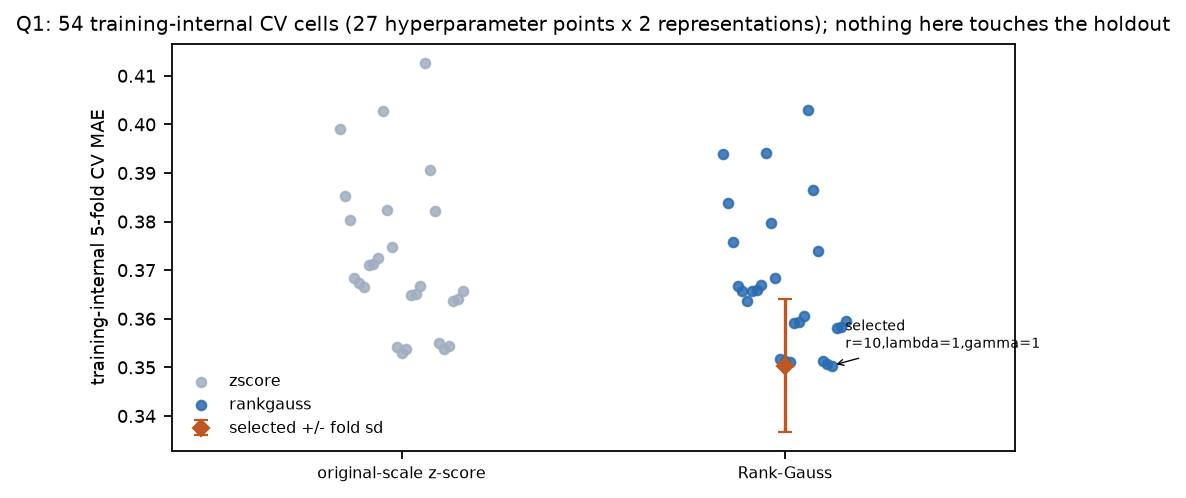
\includegraphics[keepaspectratio,alt={问题一：训练折内 5 折 CV 的 54 个格点（27 个 (r,λ,γ) 组合 × 2 种表示），纵轴为 CV MAE，灰色为原尺度 z-score、蓝色为 Rank-Gauss；橙色菱形为选中格点 r=10,λ=1,γ=1 及其折间标准差。全部超参数选择只发生在训练折内部，未接触留出集。}]{../figures/q1_cv_grid.png}}
\caption{问题一：训练折内 5 折 CV 的 54 个格点（27 个 (r,λ,γ) 组合 × 2
种表示），纵轴为 CV MAE，灰色为原尺度 z-score、蓝色为
Rank-Gauss；橙色菱形为选中格点 r=10,λ=1,γ=1
及其折间标准差。全部超参数选择只发生在训练折内部，未接触留出集。}
\end{figure}

\begin{figure}
\centering
\pandocbounded{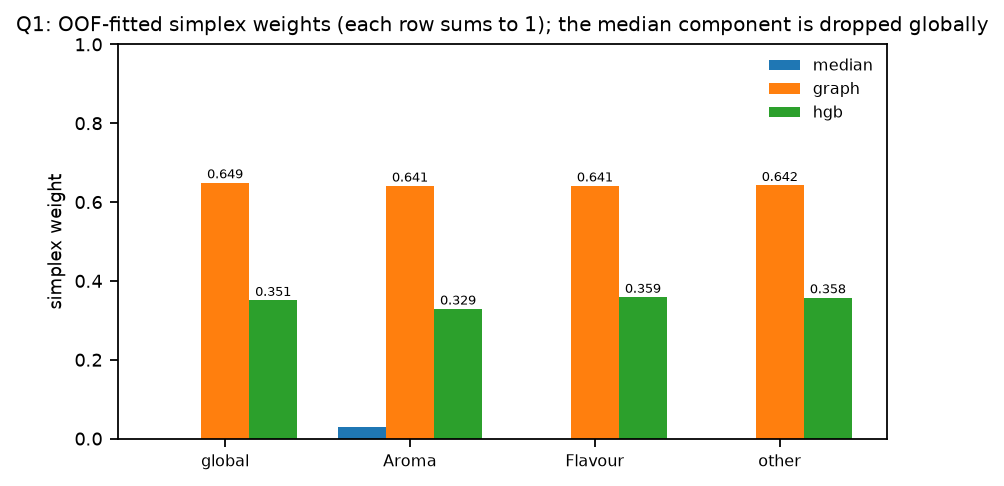
\includegraphics[keepaspectratio,alt={问题一：训练内 OOF 拟合的单纯形权重（每行三个权重之和为 1），分为全局与 Aroma/Flavour/其他三组；全局与三组都把 median 分量的权重压到接近 0，graph 约 0.64、HGB 约 0.33--0.35。}]{../figures/q1_fusion_weights.png}}
\caption{问题一：训练内 OOF 拟合的单纯形权重（每行三个权重之和为
1），分为全局与 Aroma/Flavour/其他三组；全局与三组都把 median
分量的权重压到接近 0，graph 约 0.64、HGB 约 0.33--0.35。}
\end{figure}

\subsubsection{4.4 0--6 相对分级与 250×50
交付表}\label{ux76f8ux5bf9ux5206ux7ea7ux4e0e-25050-ux4ea4ux4ed8ux8868}

3.xlsx 是\textbf{空白评分卡模板}、4.csv 是标准化连续值，``原始 0--6
人工评分''不可识别。我们显式定义相对强度等级：以训练折中点经验 CDF \[
a_{it}=\widehat F^{\mathrm{mid}}_{Y_t,\mathrm{train}}(\widehat y_{it}),\qquad g^{\mathrm{cont}}_{it}=6a_{it},\qquad g_{it}=\min\{6,\max[0,\lfloor 6a_{it}+1/2\rfloor]\},
\] 该主规则由模型契约 MCON-0001 的分段声明式公式与 7 个边界样例（覆盖
\(a=0\)、\(1/12\)、\(1/6\)、\(1/2\)、\(3/4\)、\(11/12\)、\(1\)）固定下来；敏感性分析另用训练折
5\%/95\% 分位到 0/6
的有界线性映射，仅用于检验分级对参考端点的敏感性。\textbf{等级 0
不自动表示该风味不存在，等级 6
不自动表示原人工评分满分，缺陷维度的相对高等级不等于已超过化学缺陷阈值}；标准化标签的
0 也不作为真实等级 3 的锚点。

交付层给出全部 250 行 × 50 个维度的分级表（EXP-0026 的
\texttt{grades\_all.csv}：每个维度一列 \(g^{\mathrm{cont}}\)、一列整数
\(g\)），其中 200 行训练样本为 \textbf{in-sample}、50 行留出样本为
out-of-sample。分级的二次加权 \(\kappa\) 为 0.3585644474970199、分级 MAE
为 1.3616、整级一致率为
0.236；预测被收缩会使预测级分布更集中，而参考级近均匀，因此一致率有限，这一偏差如实报告而不修饰。

\begin{figure}
\centering
\pandocbounded{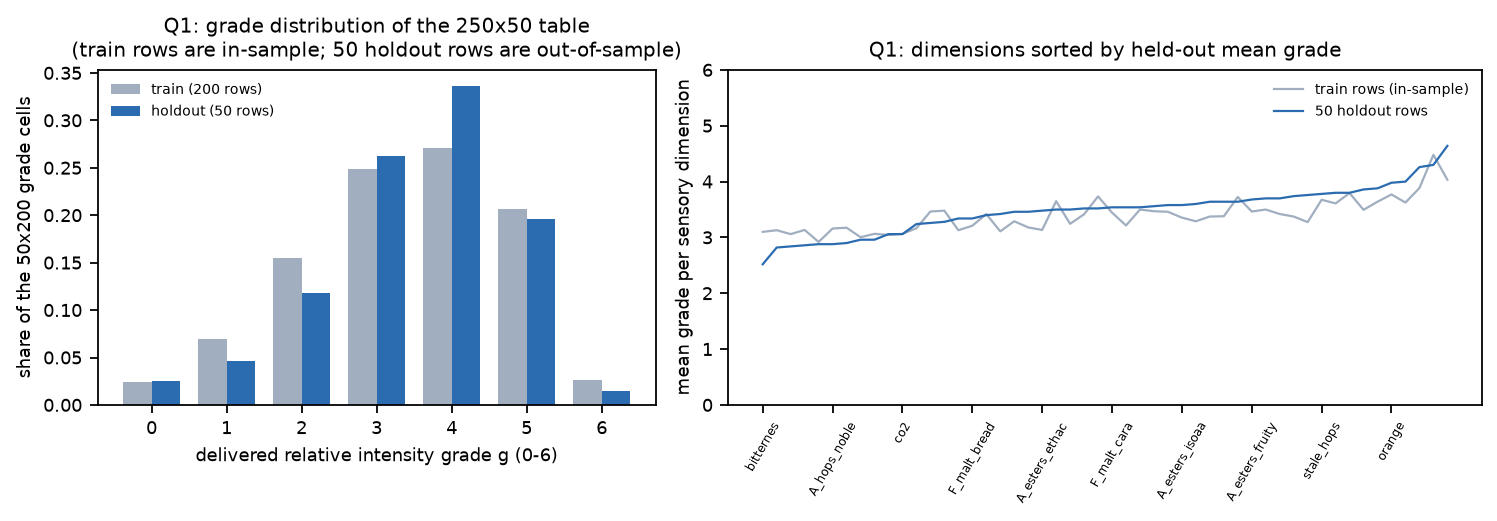
\includegraphics[keepaspectratio,alt={问题一：交付的 250×50 相对强度分级表（EXP-0026 的 grades\_all.csv）。左图为等级 0--6 的分布，200 行训练行（in-sample）与 50 行留出分别归一化；右图为按留出均值等级排序的 50 个维度在两个子集上的均值等级。等级是相对强度，0 不代表风味不存在、6 不代表人工评分满分。}]{../figures/q1_grades_all.png}}
\caption{问题一：交付的 250×50 相对强度分级表（EXP-0026 的
grades\_all.csv）。左图为等级 0--6 的分布，200 行训练行（in-sample）与
50 行留出分别归一化；右图为按留出均值等级排序的 50
个维度在两个子集上的均值等级。等级是相对强度，0 不代表风味不存在、6
不代表人工评分满分。}
\end{figure}

\subsubsection{4.5 评价与结果}\label{ux8bc4ux4ef7ux4e0eux7ed3ux679c}

以留出 50 行的真实 \(Y\) 计算逐维
\(\mathrm{MAE}_t\)、\(R_t^2\)、\(\mathrm{Skill}_t=1-\mathrm{MAE}_{t,\mathrm{model}}/\mathrm{MAE}_{t,\mathrm{median}}\)，再取
50 维等权平均：

{\def\LTcaptype{none} % do not increment counter
\begin{longtable}[]{@{}
  >{\raggedright\arraybackslash}p{(\linewidth - 6\tabcolsep) * \real{0.2000}}
  >{\raggedleft\arraybackslash}p{(\linewidth - 6\tabcolsep) * \real{0.2667}}
  >{\raggedleft\arraybackslash}p{(\linewidth - 6\tabcolsep) * \real{0.2667}}
  >{\raggedleft\arraybackslash}p{(\linewidth - 6\tabcolsep) * \real{0.2667}}@{}}
\toprule\noalign{}
\begin{minipage}[b]{\linewidth}\raggedright
实验
\end{minipage} & \begin{minipage}[b]{\linewidth}\raggedleft
50 维平均 MAE
\end{minipage} & \begin{minipage}[b]{\linewidth}\raggedleft
\(R^2_{50}\)
\end{minipage} & \begin{minipage}[b]{\linewidth}\raggedleft
Skill
\end{minipage} \\
\midrule\noalign{}
\endhead
\bottomrule\noalign{}
\endlastfoot
B0 逐目标训练中位数 & 0.4005615400064 & -0.0848384350854984 &
0（定义） \\
C1 图正则低秩回归 & 0.35455830244427766 & 0.21463819304379603 &
0.11484686613045103 \\
\textbf{C2 OOF 融合（选中）} & 0.3465674099243312 & 0.23166117909673786
& 0.13479609170966855 \\
\end{longtable}
}

C1 的训练内 CV MAE 为 0.35039761171092537（折间 sd
0.013725765669543984），明显小于基线在测试行的
MAE，说明选择过程未系统性过拟合。逐目标看，38 个维度相对基线改善、12
个维度恶化，恶化集中在训练样本极少的缺陷／风格维度；融合相对其自身分量的增益很小，多出来的那部分主要来自非线性残差而不是图结构。

\begin{figure}
\centering
\pandocbounded{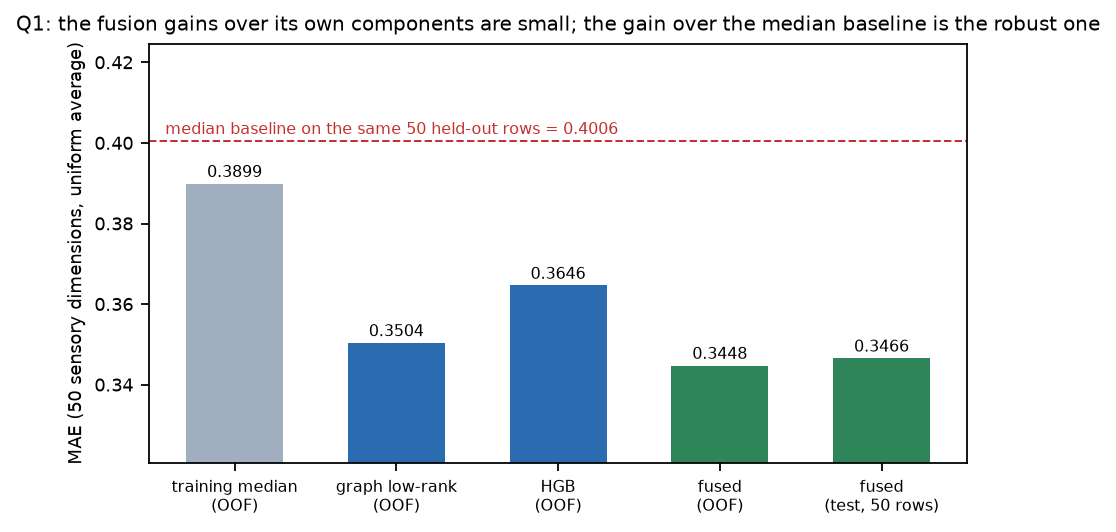
\includegraphics[keepaspectratio,alt={问题一：三个分量与融合模型的 MAE 对比。横轴依次为逐目标训练中位数（OOF）、图正则低秩回归（OOF）、HGB（OOF）、融合（OOF）、融合（50 行留出测试）；红色虚线为同一批 50 行留出上的中位数基线 MAE。融合相对自身分量的增益很小，相对中位数基线的增益才是稳健的那个。}]{../figures/q1_component_mae.png}}
\caption{问题一：三个分量与融合模型的 MAE
对比。横轴依次为逐目标训练中位数（OOF）、图正则低秩回归（OOF）、HGB（OOF）、融合（OOF）、融合（50
行留出测试）；红色虚线为同一批 50 行留出上的中位数基线
MAE。融合相对自身分量的增益很小，相对中位数基线的增益才是稳健的那个。}
\end{figure}

\begin{figure}
\centering
\pandocbounded{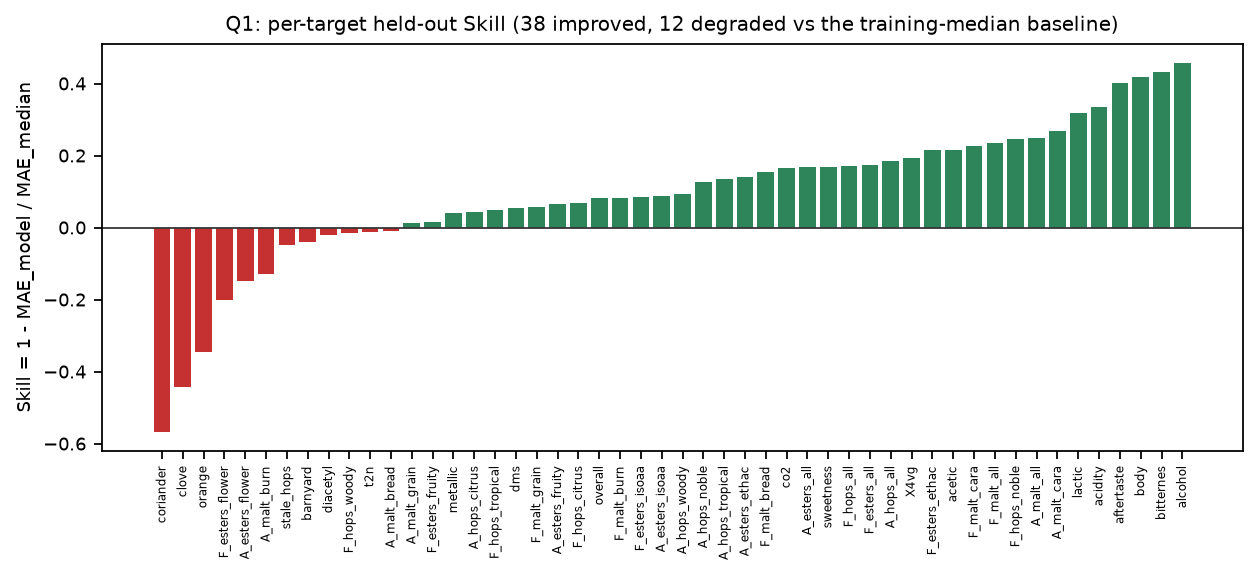
\includegraphics[keepaspectratio,alt={问题一：50 个感官维度的留出 Skill = 1 − MAE\_model/MAE\_median，按 Skill 升序排列；绿色为相对中位数基线改善的 38 维，红色为恶化的 12 维（EXP-0004 的 improvedTargets/degradedTargets）。恶化集中在训练样本极少的缺陷/风格维度。}]{../figures/q1_per_target.png}}
\caption{问题一：50 个感官维度的留出 Skill = 1 −
MAE\_model/MAE\_median，按 Skill 升序排列；绿色为相对中位数基线改善的 38
维，红色为恶化的 12 维（EXP-0004 的
improvedTargets/degradedTargets）。恶化集中在训练样本极少的缺陷/风格维度。}
\end{figure}

\subsubsection{4.6 训练内消融（第 1--3
项，负结果）}\label{ux8badux7ec3ux5185ux6d88ux878dux7b2c-13-ux9879ux8d1fux7ed3ux679c}

\begin{enumerate}
\def\labelenumi{\arabic{enumi}.}
\tightlist
\item
  \textbf{原尺度标准化 vs Rank-Gauss}：CV MAE 分别为 0.35439181724126806
  与 0.35039761171092537，差值 -0.003994205530342687；
\item
  \textbf{普通 Ridge vs 低秩约束}：0.35271965183491505 对
  0.35039761171092537，差值 0.002322040123989677；
\item
  \textbf{\(\gamma=0\) vs 图正则}：0.35138113804820575 对
  0.35039761171092537，差值 0.0009835263372803826。
\end{enumerate}

三项差值都小于折间
sd（0.013725765669543984），因此不能声称这些复杂组件带来稳定增益；真正稳定的增益来自
graph+HGB 融合（OOF 0.34476625688121565 对 graph
0.35039761171092537）。该负结果登记如下：

Q1 的三项训练内消融都只有很小的增益：Rank-Gauss 相对原尺度标准化的训练内
CV MAE 低 0.00399，普通 Ridge 相对低秩约束差 0.00232，γ=0 相对最优 γ=1
差 0.00098，三者都小于折间标准差
0.0137，因此不能声称图正则或低秩约束带来稳定增益。稳定的增益来自
graph+HGB 的 OOF 融合（OOF MAE 0.3448，graph 单模型 0.3504，差
0.0056）。这是负结果，按原样披露。

\subsection{5 问题二：共表达网络、风格混杂与稳定
Top-3}\label{ux95eeux9898ux4e8cux5171ux8868ux8fbeux7f51ux7edcux98ceux683cux6df7ux6742ux4e0eux7a33ux5b9a-top-3}

\subsubsection{5.1
两个用途不同的网络}\label{ux4e24ux4e2aux7528ux9014ux4e0dux540cux7684ux7f51ux7edc}

\begin{itemize}
\tightlist
\item
  \textbf{附件描述网络}：把 2.csv 的 231×231 Spearman
  矩阵作为登记依赖读入（EXP-0029），先做 PSD
  投影再阈值化------原始矩阵最小特征值
  -0.042412709119481015，投影后残差在 \(10^{-16}\) 量级；\(\tau=0.5\) 时
  644 条边、52 个连通块、最大块含 175 个变量。它回应题目点名要用 2.csv
  的要求，并给出附件水平的整体结构。
\item
  \textbf{训练网络}：在 200 行训练集上重算 Spearman，用于 Q1
  的图正则与任何需要评价泛化的分析。边权
  \(w_{jk}=\hat\rho_{jk}\mathbf 1\{|\hat\rho_{jk}|\ge\tau\}\)，\(\tau\in\{0.4,0.5,0.6\}\)，并用
  bootstrap 边出现频率作可靠性标注。
\end{itemize}

两者用途不同、都可在台账查证。\textbf{必须说明}：附件 2.csv 是同一批 250
款酒的关联矩阵，与 1.csv 不是独立数据源；若用全部 250
行重算图来正则化，测试信息会进入模型，因此模型侧的图只能来自训练 200
行。

\subsubsection{5.2 网络模块}\label{ux7f51ux7edcux6a21ux5757}

基于 \(|W|\) 的阈值图用连通分量识别模块 \(M_1,\dots,M_K\)，模块得分
\(m_{ik}=\mathrm{PC1}(Z_{i,M_k})\)，先分析模块与感官维度的关系，再解释模块内候选。\(\tau=0.5\)
时有 51
个连通块，但最大块几乎吞并了全部特征（传递连通），模块区分度弱；\(\tau=0.6\)
时给出 108 块、291
条边的更严划分，两者都报告。因此模块只作为解释线索，\textbf{不进入 Top-3
打分}。

\begin{figure}
\centering
\pandocbounded{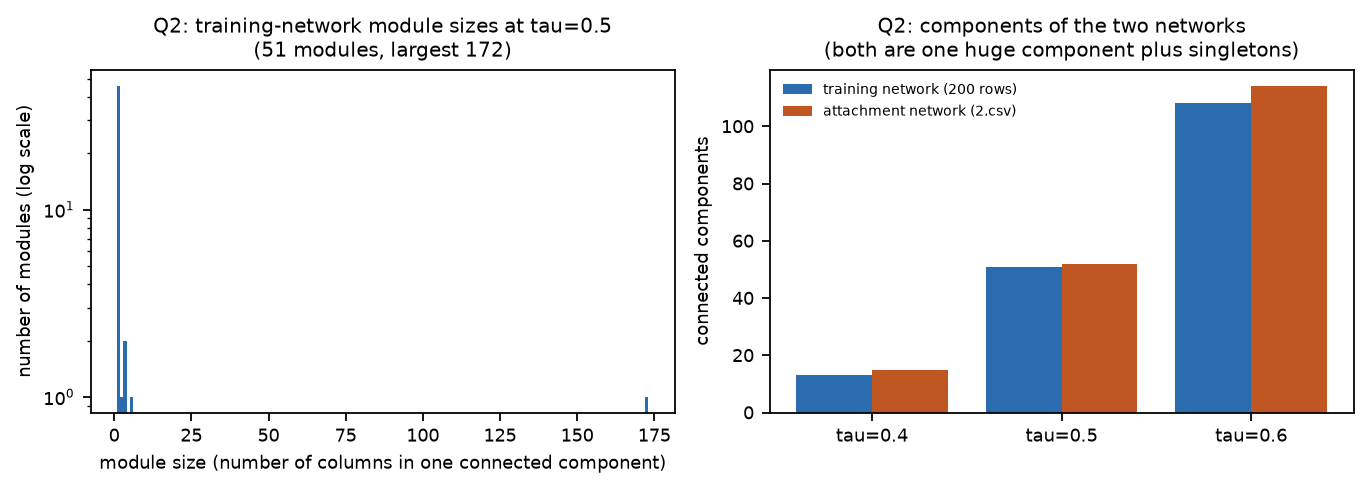
\includegraphics[keepaspectratio,alt={问题二：左图为训练网络（τ=0.5）的模块规模分布（纵轴对数），51 个连通块、最大块含 172 列；右图为训练网络（200 行重算）与附件 2.csv 网络（PSD 投影后阈值化）在 τ=0.4/0.5/0.6 下的连通分量数对比------两者都是``一个巨大连通块 + 大量单点''，模块区分度弱，因此模块只作解释线索而不进入 Top-3 打分。}]{../figures/q2_modules.png}}
\caption{问题二：左图为训练网络（τ=0.5）的模块规模分布（纵轴对数），51
个连通块、最大块含 172 列；右图为训练网络（200 行重算）与附件 2.csv
网络（PSD 投影后阈值化）在 τ=0.4/0.5/0.6
下的连通分量数对比------两者都是``一个巨大连通块 +
大量单点''，模块区分度弱，因此模块只作解释线索而不进入 Top-3 打分。}
\end{figure}

\subsubsection{5.3
总体关联与风格内关联}\label{ux603bux4f53ux5173ux8054ux4e0eux98ceux683cux5185ux5173ux8054}

总体关联
\(\rho^{\mathrm{total}}_{jt}=\operatorname{Spearman}(X_j,Y_t)\)；风格内关联先对秩作风格虚拟变量与截距的残差化：
\[
r_j^X=\big[I-H(H^\top H)^\dagger H^\top\big]\operatorname{rank}(X_j),\quad r_t^Y=\big[I-H(H^\top H)^\dagger H^\top\big]\operatorname{rank}(Y_t),\quad \rho^{\mathrm{within}}_{jt}=\operatorname{Corr}(r_j^X,r_t^Y).
\]
据此区分四类：总体与风格内均稳定、主要体现风格差异、被风格差异遮蔽、不同风格方向不一致。第
4 项消融（总体 vs 风格内）见第 8 节。

\subsubsection{\texorpdfstring{5.4 固定的综合规则与``\(\pi\)
优先''的最终
Top-3}{5.4 固定的综合规则与``\textbackslash pi 优先''的最终 Top-3}}\label{ux56faux5b9aux7684ux7efcux5408ux89c4ux5219ux4e0epi-ux4f18ux5148ux7684ux6700ux7ec8-top-3}

对实际单体化合物候选（219 个），定义 \[
S_{jt}=\frac13\Big[R\big(|\rho^{\mathrm{total}}_{jt}|\big)+R\big(|\rho^{\mathrm{within}}_{jt}|\big)+R\big(|\widehat B_{jt}|\big)\Big],
\] 其中 \(R\) 是列内``越大越高''的百分位，\(\widehat B\) 来自与 Q1
同族的图正则低秩回归（\(\tau=0.5,\lambda=1,\gamma=0.1,r=6\)，不调参）。进行
\(B=500\) 次风格分层
bootstrap（每个风格内有放回重采样到该风格样本数；每次重拟合秩变换、网络与模型），得到
\[
\pi_{jt}=\frac1B\sum_{b=1}^B\mathbf 1\{j\in\operatorname{Top3}^{(b)}_t\}.
\]

\textbf{交付的最终 Top-3 严格按蓝图 §4.4 的规则排序：先按 \(\pi_{jt}\)
降序，\(\pi\) 相同时用平均综合分 \(S_{jt}\)
裁决并列}（\texttt{sets\_pi\_first.json} 与 \texttt{outputs.final\_top3}
逐维给出 \(\pi\)、\(S\) 分量、方向、模块与风格混杂标签）。主指标
\texttt{topk-jaccard} 仍按注册口径由三种单方法集合与``按 \(S\) 取前
3''的综合集合的 \texttt{sets.json} 复算，这一口径下值为
0.21866666666666665；若把综合集合换成 \(\pi\) 优先集合，同一指标为
0.24，两个数同时报告，不以后者替换已注册的主指标。点估计综合集与 \(\pi\)
优先集在 24 个维度上不同，Jaccard 为
0.736------这正是必须同时报告两者的原因。

\subsubsection{5.5
结果与化学合理性}\label{ux7ed3ux679cux4e0eux5316ux5b66ux5408ux7406ux6027}

{\def\LTcaptype{none} % do not increment counter
\begin{longtable}[]{@{}lr@{}}
\toprule\noalign{}
方法／基线 & topk-jaccard \\
\midrule\noalign{}
\endhead
\bottomrule\noalign{}
\endlastfoot
维度无关的全局 Top-3 基线 & 0.19999999999999996 \\
\textbf{四方法逐维 Top-3（选中）} & 0.21866666666666665 \\
\end{longtable}
}

500 次 bootstrap 下交付 Top-3 的 \(\pi\) 均值为
0.46468，没有任何化合物达到 \(\pi=1\)，说明单维 Top-3
存在实质竞争；这是把 \(\pi\) 作为稳定性主证据、并用 \(S\)
裁决并列的原因。方法间 Jaccard 见本节末图：总体与风格内两种关联的
Jaccard 只有
0.302，说明\textbf{风格混杂确实改变``哪些化合物最重要''的答案}；图正则系数与另两种排序的
Jaccard 最低（图中最矮的两条边）。

每个最终候选记录
\(\{\)方向、强度、\(\pi\)、模块、风格混杂、化学解释、证据等级\(\}\)。与
6.csv 的独立 \(|r|\) 在 44/44 个化合物上对齐后，50 维秩相关均值为
0.44505144467935176；7.csv 的跨来源描述符与 8.xlsx 的 GBM
importance/SHAP
只作非独立对照，不参与选择。主结论登记如下（只声明同期关联，不宣称因果或未来预测）：

在 200 行训练集上，以附件 2.csv 的 231×231 Spearman 矩阵（PSD
投影：原始最小特征值 −0.0424，τ=0.5 时 644 条边、52
个连通块）为附件描述网络、以训练集重算的 Spearman 图为正则化网络，50 维
× 4 方法 Top-3 的平均两两 Jaccard 为 0.219（可由 sets.json
原样复算），维度无关的全局 Top-3 基线为 0.20。500 次风格分层 bootstrap
下交付 Top-3 的入选频率均值 0.465、没有任何化合物达到 π=1。最终 Top-3
按蓝图 §4.4「π 优先、平均综合分 S
裁决并列」给出（sets\_pi\_first.json）；把四个方法的 Top-3 全部换成 π
优先重选结果后，同一 Jaccard 为 0.24，而点估计综合集口径仍为
0.219，两者同时报告、不互相替换；π 优先集与点估计综合集的 Jaccard 为
0.736。与 6.csv 独立 \textbar r\textbar{} 的秩相关均值 0.445（44/44
化合物对齐）只支持方向一致性，不等同独立验证。只声明同期关联，不宣称因果或未来预测。

\begin{figure}
\centering
\pandocbounded{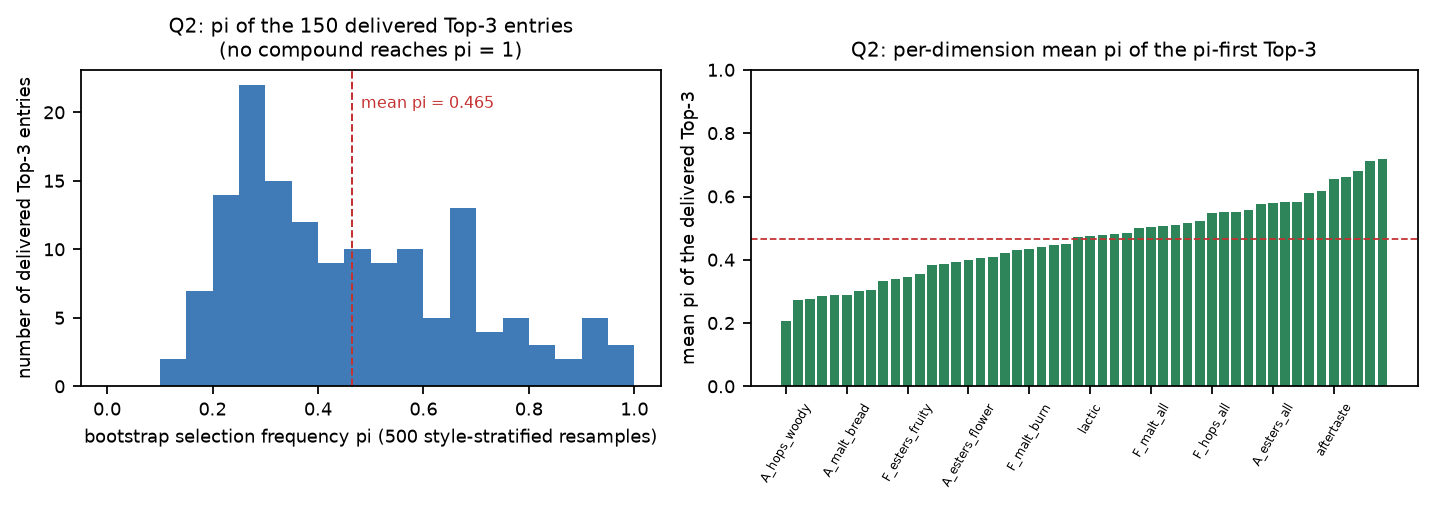
\includegraphics[keepaspectratio,alt={问题二：500 次风格分层 bootstrap 下交付 Top-3 的入选频率 π。左图为 150 个交付条目的 π 分布（均值 0.465，没有任何化合物达到 π=1），右图为 50 个维度各自的平均 π（按 π 排序）；这是把 π 作为稳定性主证据、并用平均综合分 S 裁决并列的依据。}]{../figures/q2_bootstrap_pi.png}}
\caption{问题二：500 次风格分层 bootstrap 下交付 Top-3 的入选频率
π。左图为 150 个交付条目的 π 分布（均值 0.465，没有任何化合物达到
π=1），右图为 50 个维度各自的平均 π（按 π 排序）；这是把 π
作为稳定性主证据、并用平均综合分 S 裁决并列的依据。}
\end{figure}

\begin{figure}
\centering
\pandocbounded{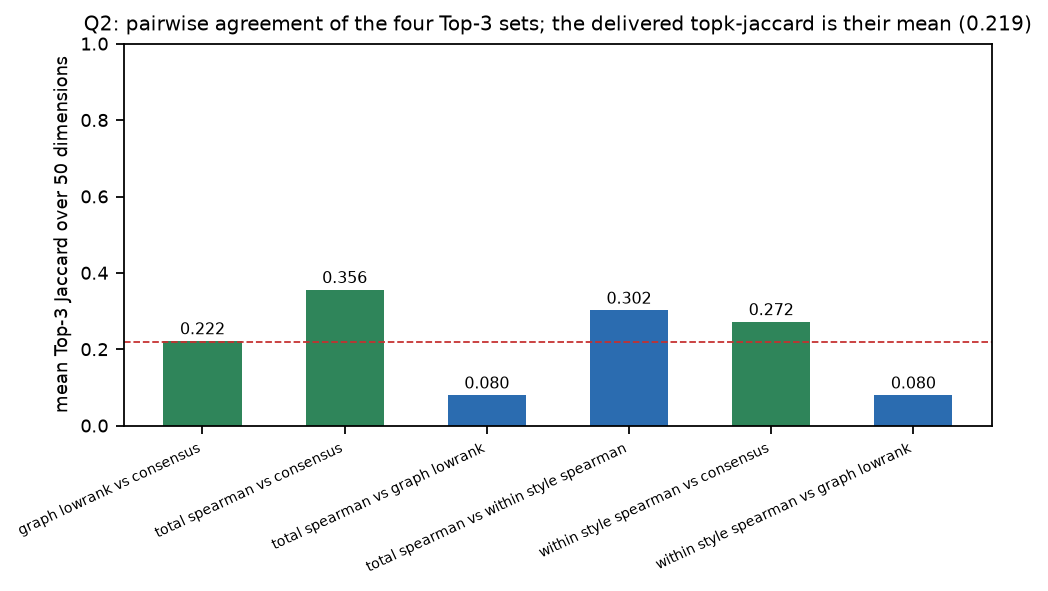
\includegraphics[keepaspectratio,alt={问题二：四种方法（总体 Spearman、风格内 Spearman、图正则低秩 \textbar B\textbar、综合分 S）Top-3 集合两两 Jaccard 系数的 50 维平均；红色虚线为四种方法两两平均的主指标 topk-jaccard=0.219。总体与风格内两种关联的 Jaccard 仅 0.302（6 条边中最接近的两条），图正则系数与另两种排序的 Jaccard 只有 0.080。}]{../figures/q2_method_jaccard.png}}
\caption{问题二：四种方法（总体 Spearman、风格内 Spearman、图正则低秩
\textbar B\textbar、综合分 S）Top-3 集合两两 Jaccard 系数的 50
维平均；红色虚线为四种方法两两平均的主指标
topk-jaccard=0.219。总体与风格内两种关联的 Jaccard 仅 0.302（6
条边中最接近的两条），图正则系数与另两种排序的 Jaccard 只有 0.080。}
\end{figure}

\subsection{6
问题三：风格条件生成与跨风格迁移}\label{ux95eeux9898ux4e09ux98ceux683cux6761ux4ef6ux751fux6210ux4e0eux8de8ux98ceux683cux8fc1ux79fb}

\subsubsection{6.1
风格内留出协议}\label{ux98ceux683cux5185ux7559ux51faux534fux8bae}

主任务学习\textbf{已有目标风格}：用目标风格已有训练样本学习
\(p(X\mid s)\)，在风格内部留出真实样本（固定 3
折，\texttt{data/clean/q3\_style\_protocol.json}），共 250 行
out-of-fold 生成；Tripel、Kriek、Lambic 整类排除训练（49
行）仅作为\textbf{未见风格泛化扩展}，单独报告，绝不与主分数合并。4.csv
的 50 个标签只用于评估，不进入生成模型似然。

\subsubsection{6.2 风格收缩边际与 floor
混合}\label{ux98ceux683cux6536ux7f29ux8fb9ux9645ux4e0e-floor-ux6df7ux5408}

\[
\widehat F_{j,s}=\omega_s\widehat F^{\mathrm{emp}}_{j,s}+(1-\omega_s)\widehat F^{\mathrm{pool}}_j,\qquad \omega_s=\frac{n_s}{n_s+\kappa},\quad \kappa\in\{0,5,15\}.
\] 有地板编码的变量使用观测混合分布 \[
F^{\mathrm{obs}}_{j,s}(v)=\pi^{\mathrm{floor}}_{j,s}\mathbf 1\{v\ge v_j^{\mathrm{floor}}\}+(1-\pi^{\mathrm{floor}}_{j,s})F^{\mathrm{nonfloor}}_{j,s}(v),
\] 采样时以 \(\pi^{\mathrm{floor}}\) 概率取 floor 原子、否则从非 floor
子样本经验 CDF 采样。最终 \(\kappa\) 由训练内风格半折 CV 的 9
个格点跨折均值 argmin 选出（并列取更强收缩），得 \(\kappa=\) 5。

\subsubsection{6.3 Copula
依赖结构}\label{copula-ux4f9dux8d56ux7ed3ux6784}

\[
z_{ij}=\Phi^{-1}\big[\widehat F_{j,s_i}(x_{ij})\big],\qquad \widehat R_s=\eta_s\widehat R_s^{\mathrm{emp}}+(1-\eta_s)\widehat R_{\mathrm{shared}},\quad \eta_s=\frac{n_s}{n_s+\kappa_R}.
\] 相关矩阵特征值截断到 \(\ge10^{-6}\)、归一化后再向单位阵收缩 5\%，采样
\(z^*\sim N(0,\widehat R_s)\Rightarrow u_j^*=\Phi(z_j^*)\Rightarrow x_j^*=\widehat F_{j,s}^{-1}(u_j^*)\)；对已确认尺度的变量再转成
\(c_j^*\) 检查阈值。最终 \(\kappa_R=\) 20。

\subsubsection{6.4
三层检查与低缺陷生成}\label{ux4e09ux5c42ux68c0ux67e5ux4e0eux4f4eux7f3aux9677ux751fux6210}

\textbf{观测分布合理性}用固定训练集标准化表示上的归一化能量距离 \[
\mathcal E^2=2\mathbb E\|X-Y\|-\mathbb E\|X-X'\|-\mathbb E\|Y-Y'\|,\qquad \mathcal E_{\mathrm{norm}}=\sqrt{\max(\mathcal E^2,0)/D_{\mathrm{ref}}},
\] \(D_{\mathrm{ref}}\)
为同量真实训练样本的典型两两距离，并提供同量真实---真实参照。\textbf{物理有效性}检查非负、训练支撑与派生量一致性；\textbf{缺陷风险}检查
3 个有阈值缺陷（DMS 17.25 μg/L、双乙酰 0.29925 mg/L、4VG 0.206333
mg/L，取 8.xlsx 均值，阈值登记在
\texttt{data/clean/q3\_thresholds.json}）与 t2n
的风格上界。普通条件生成与低缺陷生成（对有阈值缺陷施加
\(e_j(c)=\max(c_j/T_j-1,0)=0\)，t2n 用风格训练 q90 上界）分别评价。

结果为：低缺陷生成的约束满足率 1（250 行 OOF 生成 + 49 行未见风格 + 11
行迁移，全部满足 MCON-0003 的五条约束），未约束生成仅
0.136，无条件全局高斯基线 0.12；缺陷超阈率方面，未约束生成
0.852、真实数据 0.844、低缺陷生成
0。约束投影的代价很小：\(\mathcal E_{\mathrm{norm}}\) 由
0.23111037792411374 变为 0.23521270840867994（真实---真实参照
0.18418128739199716；无条件基线
0.7513853833897858）。逐风格的能量距离见本节末图：未见风格扩展的
\(\mathcal E_{\mathrm{norm}}\) 为 0.3590035848831178，Tripel 较好而
Kriek/Lambic 区间很宽，小样本如实披露。

经 Q1 代理的 50 维合并感官画像 Spearman 为 0.7963025210084033、MAE 为
0.01450187654791753；但逐风格图（第 6.4
节末）显示这一合并分数掩盖了逐风格异质（Amber 为负、Brut 与
Brett/cofermented 接近 0、Kriek 与 Strong ale
较高），因此\textbf{合并分数不能读成逐风格可靠}，t2n/stale hops 的代理
CV \(R^2\) 仅
0.0548889784422808/0.05025260385796093，相关结论只作弱证据。

\begin{figure}
\centering
\pandocbounded{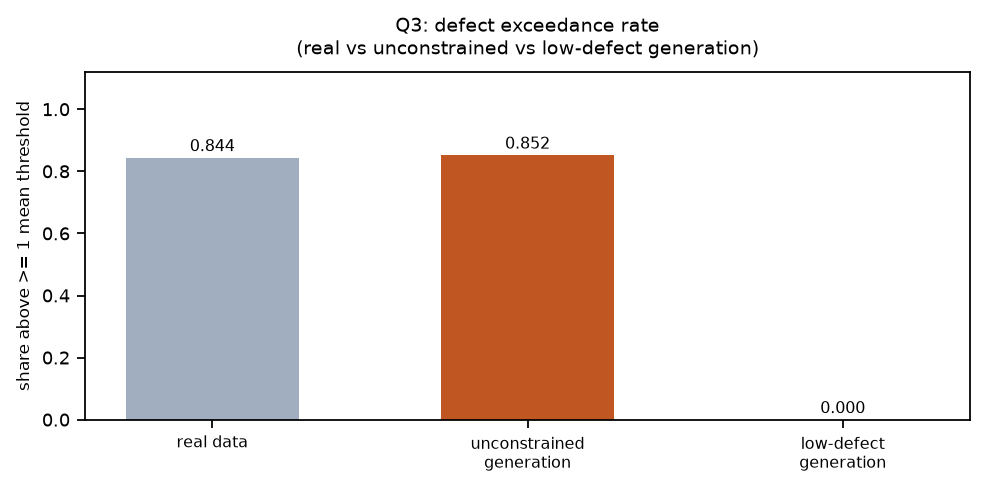
\includegraphics[keepaspectratio,alt={问题三：至少一种均值阈值缺陷超阈的样本比例------真实数据 0.844、未约束条件生成 0.852、低缺陷生成 0.000。约束把缺陷超阈率降到 0，而生成模型在加约束前的缺陷水平与真实数据相当。}]{../figures/q3_defect_exceedance.png}}
\caption{问题三：至少一种均值阈值缺陷超阈的样本比例------真实数据
0.844、未约束条件生成 0.852、低缺陷生成 0.000。约束把缺陷超阈率降到
0，而生成模型在加约束前的缺陷水平与真实数据相当。}
\end{figure}

\begin{figure}
\centering
\pandocbounded{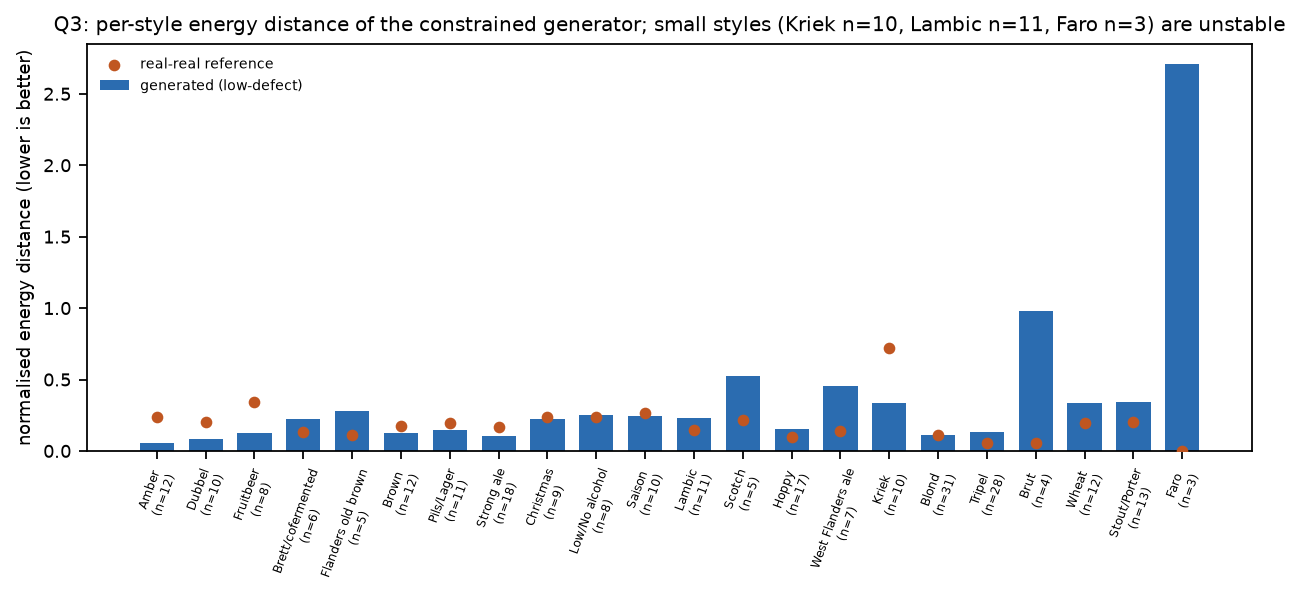
\includegraphics[keepaspectratio,alt={问题三：约束生成在 22 个风格上的归一化能量距离（蓝柱，按风格留出样本量加权）与同样本量的真实---真实参照（橙点）；Kriek (n=10)、Lambic (n=11)、Faro (n=3) 等小风格波动很大，不声称精确刻画。}]{../figures/q3_energy_by_style.png}}
\caption{问题三：约束生成在 22
个风格上的归一化能量距离（蓝柱，按风格留出样本量加权）与同样本量的真实---真实参照（橙点）；Kriek
(n=10)、Lambic (n=11)、Faro (n=3) 等小风格波动很大，不声称精确刻画。}
\end{figure}

\begin{figure}
\centering
\pandocbounded{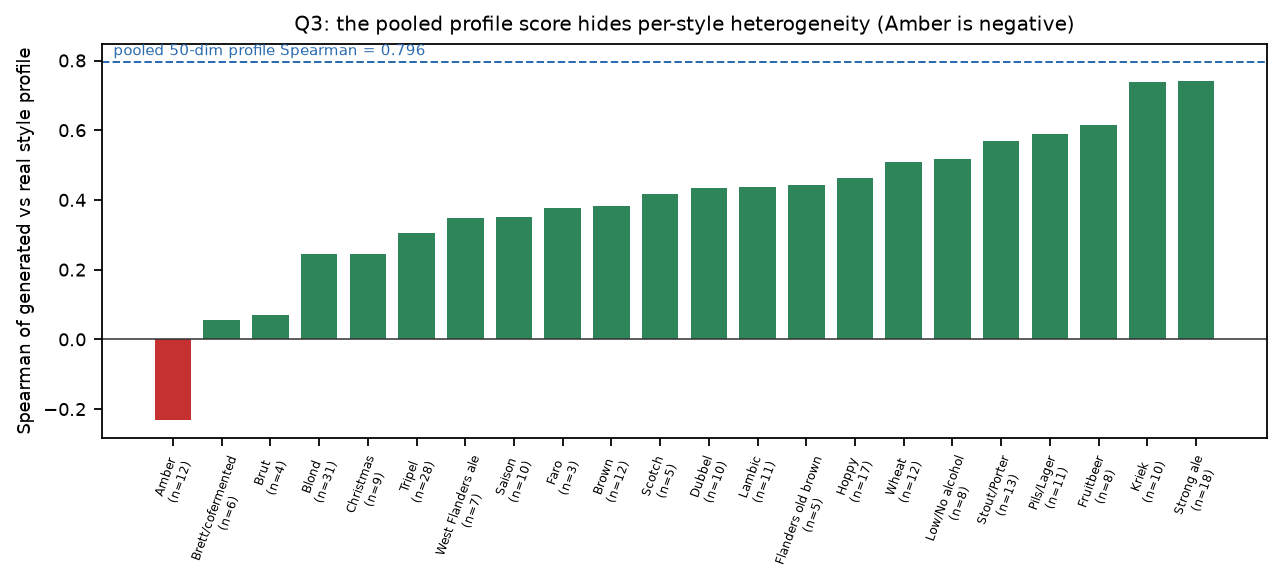
\includegraphics[keepaspectratio,alt={问题三：生成谱经 Q1 感官代理映射后的 50 维感官画像与同风格真实留出样本画像的 Spearman 相关，按风格排列（横轴标注样本量）；蓝色虚线为合并口径的 0.796。逐风格异质性明显：Amber (n=12) 为负、Brut (n=4) 与 Brett/cofermented (n=6) 接近 0，Kriek (n=10) 与 Strong ale (n=18) 较高，因此合并分数不能读成逐风格可靠。}]{../figures/q3_profile.png}}
\caption{问题三：生成谱经 Q1 感官代理映射后的 50
维感官画像与同风格真实留出样本画像的 Spearman
相关，按风格排列（横轴标注样本量）；蓝色虚线为合并口径的
0.796。逐风格异质性明显：Amber (n=12) 为负、Brut (n=4) 与
Brett/cofermented (n=6) 接近 0，Kriek (n=10) 与 Strong ale (n=18)
较高，因此合并分数不能读成逐风格可靠。}
\end{figure}

\subsubsection{6.5 跨风格迁移：分位数初始化 +
最小改动约束优化}\label{ux8de8ux98ceux683cux8fc1ux79fbux5206ux4f4dux6570ux521dux59cbux5316-ux6700ux5c0fux6539ux52a8ux7ea6ux675fux4f18ux5316}

分位数映射给出初始化 \[
x_j^{(0)}=\widehat F_{j,\mathrm{Tripel}}^{-1}\big[\widehat F_{j,\mathrm{Pils/Lager}}(x_j^{\mathrm{source}})\big].
\] 在单调规范化坐标 \(v_j=h_j(x_j)\in[0,1]\) 与低维表示
\(a=A(v-\mu_T)\)（Tripel 训练集 PCA 前 10 主成分）下求解 \[
\min_v\ (v-v^{(0)})^\top Q(v-v^{(0)})+\lambda D_{\mathrm{target}}(v)+\eta\|D(v-v^{\mathrm{source}})\|_1
\] 满足物理边界、缺陷不恶化、派生量关系与可信变动范围，其中
\(D_{\mathrm{target}}(v)=(Av-\mu_T)^\top\Sigma_T^{-1}(Av-\mu_T)\)、\(\Sigma_T=0.9\Sigma_T^{\mathrm{emp}}+0.1I\)。优化变量为
\(v\in[0,1]^{231}\)，用 L-BFGS-B，缺陷硬约束用可行域投影（每步把
DMS/双乙酰/4VG 的存储值投影到约束上界，t2n 与 stale hops 用 Q1
感官代理平移）。

\begin{itemize}
\tightlist
\item
  \textbf{两种不恶化策略}：超阈不恶化
  \(c_j^{\mathrm{new}}\le\max(c_j^{\mathrm{source}},T_j)\) 与绝对不增
  \(c_j^{\mathrm{new}}\le c_j^{\mathrm{source}}\)；
\item
  \textbf{双阈值情景}：\(T_j\) 分别取 8.xlsx 的 mean 与 median；
\item
  \textbf{题目指定缺陷}：DMS、双乙酰、4VG 用阈值；t2n 无阈值，施加
  \(c_{\mathrm{t2n}}^{\mathrm{new}}\le c_{\mathrm{t2n}}^{\mathrm{source}}\)；stale
  hops 是感官维度，用 Q1 代理筛查并报告不确定性。
\end{itemize}

结果：\textbf{必须分清两个口径}。策略相对非恶化率由可行域投影构造保证、不是经验发现；严格逐缺陷不增率在「绝对不增」策略下由
\(c^{\mathrm{new}}\le c^{\mathrm{source}}\)
同一约束直接保证，在「超阈不恶化」（cap-at-max）策略下则明显更低，逐缺陷拆分见
EXP-0033 的 \texttt{outputs.transfer-scenarios}；对 t2n/stale
两个代理约束的标签代理重抽样只给出代理口径的分位，不是五类缺陷严格率的下界。Pareto
前沿（\(\lambda\in\{0.1,1,10\}\times\eta\in\{0,0.01,0.1\}\)）见本节末图：\(\lambda\)
越大目标越近、改动越大，\(\eta\) 只带来很小额外代价，9
个格点的非恶化率全部与可行域允许的最大值一致。\textbf{两种策略的差别是约束保证的强度}（严格不增
vs 不超过
\(\max(c^{\mathrm{source}},T)\)），而不是可行性或代价；具体数值与逐缺陷拆分见紧随其后的登记结论。迁移结论登记如下：

Pils/Lager→Tripel 迁移中，两种策略的\textbf{策略相对}非恶化率都是
1.0，两种策略在「绝对不增」与 cap-at-max
下的严格性差异如下：绝对不增策略（c\_new≤c\_source）的严格逐缺陷不增率为
1.000，cap-at-max 策略（c\_new≤max(c\_source,T)）的\textbf{严格达标率}为
0.1818（逐缺陷：DMS 0.2727、2,3-butanedione 0.5455（mean
阈值）/0.7273（median 阈值）、4VG 0.4545；t2n 与 stale\_hops 为 1.0
但两者是 Q1 线性代理，CV R² 0.055/0.050）。四种情景的可行率都是
1.000，平均 L1
改动与目标马氏距离几乎相同，因此两种策略的差别是\textbf{约束保证的强度}（严格不增
vs 不超过 max(source,T)），而不是可行性或代价上的张力；0.1818 描述的是
cap-at-max 输出的严格达标比例，不能读成「只有 18.18\%
的源样本存在严格不增可行解」。对 t2n/stale 两个代理约束做 100
次标签代理重抽样，其联合非恶化率的 2.5\% 分位为
0.2727（代理口径，不是五类缺陷严格率的下界）。约束优化把到 Tripel
的马氏距离由分位数初始化的 1.481 降到 0.433，平均 L1 改动 7.19；mean 与
median 两套阈值情景的目标距离几乎相同。

\begin{figure}
\centering
\pandocbounded{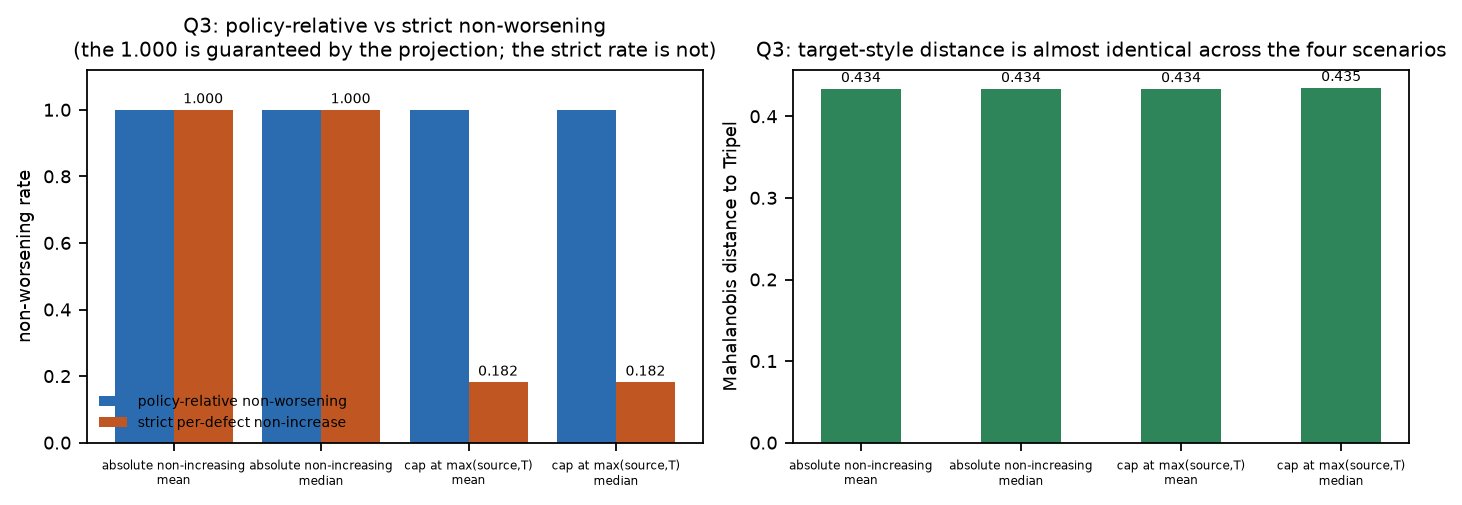
\includegraphics[keepaspectratio,alt={问题三：Pils/Lager→Tripel 的 4 个迁移情景（2 种非恶化策略 × mean/median 两套阈值）。左图为策略相对非恶化率（四种情景恒为 1.000，由投影构造保证）与严格逐缺陷不增率（绝对不增策略为 1.000，cap-at-max 策略仅 0.182）；右图为目标风格马氏距离，四种情景几乎相同（0.434--0.435），说明阈值情景的选择对目标接近度影响很小。}]{../figures/q3_transfer_scenarios.png}}
\caption{问题三：Pils/Lager→Tripel 的 4 个迁移情景（2 种非恶化策略 ×
mean/median 两套阈值）。左图为策略相对非恶化率（四种情景恒为
1.000，由投影构造保证）与严格逐缺陷不增率（绝对不增策略为
1.000，cap-at-max 策略仅
0.182）；右图为目标风格马氏距离，四种情景几乎相同（0.434--0.435），说明阈值情景的选择对目标接近度影响很小。}
\end{figure}

\begin{figure}
\centering
\pandocbounded{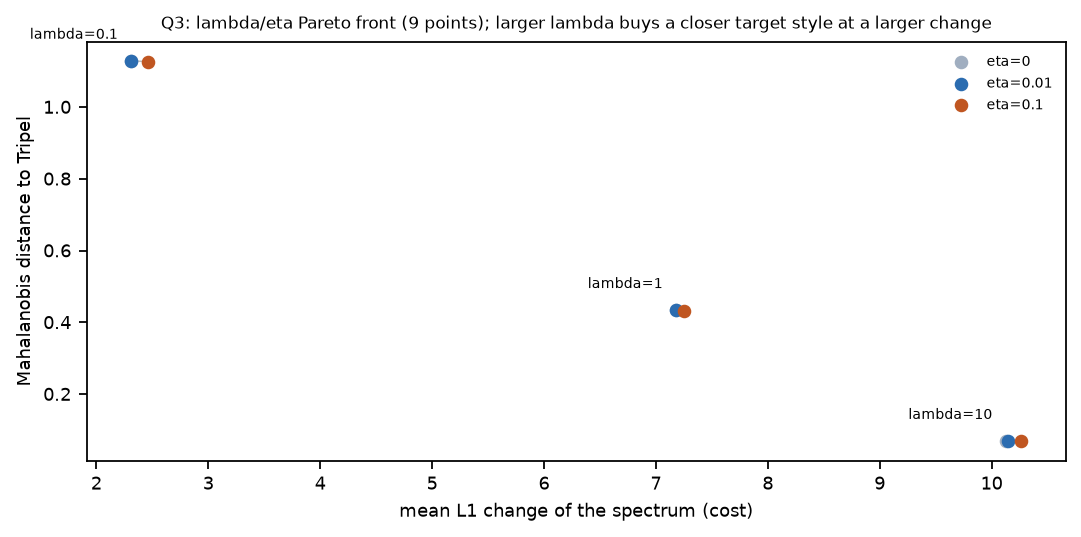
\includegraphics[keepaspectratio,alt={问题三：λ\textbackslash in\{0.1,1,10\} × η\textbackslash in\{0,0.01,0.1\} 共 9 个格点的 Pareto 前沿（横轴为平均 L1 改动量，纵轴为到 Tripel 的马氏距离，越小越接近目标风格）；灰线连接同一 λ 的三个 η 变体，颜色区分 η，每个 λ 只标注一次。λ 越大目标风格越近、谱改动越大，η 只带来很小的额外代价，9 个格点的非恶化率全部与可行域允许的最大值一致。}]{../figures/q3_pareto.png}}
\caption{问题三：λ\(\in\)\{0.1,1,10\} × η\(\in\)\{0,0.01,0.1\} 共 9
个格点的 Pareto 前沿（横轴为平均 L1 改动量，纵轴为到 Tripel
的马氏距离，越小越接近目标风格）；灰线连接同一 λ 的三个 η 变体，颜色区分
η，每个 λ 只标注一次。λ 越大目标风格越近、谱改动越大，η
只带来很小的额外代价，9 个格点的非恶化率全部与可行域允许的最大值一致。}
\end{figure}

\subsubsection{6.6 生成模型消融（第 5--9
项）}\label{ux751fux6210ux6a21ux578bux6d88ux878dux7b2c-59-ux9879}

\begin{enumerate}
\def\labelenumi{\arabic{enumi}.}
\setcounter{enumi}{4}
\tightlist
\item
  \textbf{独立边际 vs Copula}：独立边际的 \(\mathcal E_{\mathrm{norm}}\)
  反而低 -0.007951703102091506，但依赖结构谱 MAE 由 0.006302743822556374
  升至 0.015088948876474674------能量距离对 Copula 不敏感，Copula
  的收益体现在依赖结构，不能只报 \(\mathcal E_{\mathrm{norm}}\)；
\item
  \textbf{无收缩（\(\kappa=0,\kappa_R=0\)）vs 收缩}：无收缩
  \(\mathcal E_{\mathrm{norm}}\) 高 0.03365453839186214，收缩有效；
\item
  \textbf{不考虑编码质量点 vs 混合边际}：去掉 floor
  原子最伤，\(\mathcal E_{\mathrm{norm}}\) 高 0.33984476030610344；
\item
  \textbf{普通生成 vs 低缺陷生成}：约束后 \(\mathcal E_{\mathrm{norm}}\)
  只差 -0.004102330484566208（代价小），缺陷超阈率由 0.852 降到 0；
\item
  \textbf{分位数迁移 vs 约束优化}：目标马氏距离由 1.4813209885603504
  降到 0.4328202679486975。
\end{enumerate}

\subsection{7
验证设计与稳健性（含失败与限制披露）}\label{ux9a8cux8bc1ux8bbeux8ba1ux4e0eux7a33ux5065ux6027ux542bux5931ux8d25ux4e0eux9650ux5236ux62abux9732}

\textbf{协议先于比较}：在登记任何候选之前，三问各登记且仅登记一个验证计划（Q1：split-integrity、leakage、holdout-metrics、baseline-compare、independent-rerun；Q2：leakage、holdout-metrics、independent-rerun；Q3：leakage、holdout-metrics、simulation-seeds、independent-rerun）。检查由插件原生重算：Q1
的 50 维 MAE 由注册预测文件与测试真值复算（VAL-0034）、Q2 的
topk-jaccard 由 \texttt{sets.json} 复算（VAL-0038）、Q3 的
constraint-satisfaction 由 \texttt{samples.csv} 与 MCON-0003
的五条数值约束复算（VAL-0041），三者的复算值与实验记录值之差都在机器精度量级；三问的独立复跑都用\textbf{新实验
id} 在固定 seed 下逐项比较全部数值指标（VAL-0036 / VAL-0039 /
VAL-0043，全部在声明的容差内复现，逐项比较见各 VAL 的
\texttt{result.json}）。

\textbf{Holdout 预算}：SPLIT-0002 共 5 条实验记录 = \textbf{3
次模型曝光}（EXP-0001 基线、EXP-0003 C1、EXP-0004 C2）＋ \textbf{2 次
verified rerun}（EXP-0010、EXP-0025，按 \texttt{verifiedRerun}
不计曝光；其中只有 EXP-0010 有独立复跑验证记录，见
VAL-0005/VAL-0031/VAL-0036，EXP-0025 是台账中第二条未单独验证的 verified
rerun）。每行曝光 3 次，达到 \texttt{maxHoldoutReuse:\ 3}
上限，之后不再在该划分上注册任何非复跑实验；Q1
的稳健性扰动（EXP-0016--0018）与 Q2 的（EXP-0019--0021）只用
\texttt{SPLIT-0001/train.csv} 作依赖、不挂
split，因此不消耗曝光。SPLIT-0001 不挂载任何正式评估实验，其训练行被
Q1/Q2 的稳健性与 Q2 的关联分析使用。

\textbf{失败与回退（按原样保留，不删除、不改写）}：

\begin{enumerate}
\def\labelenumi{\arabic{enumi}.}
\tightlist
\item
  \textbf{EXP-0012 → failed}（\texttt{SEED\_NOT\_ACKNOWLEDGED}）：Q3
  候选为绕开 simulation-seeds 把 \texttt{seed-receipt.json} 误读成逐
  seed 运行文件的问题，把 receipt 改名为
  \texttt{env-seed.json}，但该次注册仍声明
  \texttt{requireSeedReceipt:true}，runner 找不到 receipt
  即失败。修复：Q3 候选不再声明该参数（EXP-0013 起成功），稳健性实验保留
  receipt 并声明 \texttt{true}。
\item
  \textbf{VAL-0011 → passed=false}（EXP-0009 的
  simulation-seeds）：\texttt{run.json}/\texttt{seed-receipt.json}
  被正则当成第 4 个 run 且无指标。修复后 VAL-0012 与
  VAL-0015/VAL-0029/VAL-0042 通过。
\item
  \textbf{VAL-0020 → passed=false}（EXP-0028 的
  leakage，\texttt{feature-set-unknown}）：EXP-0028 注册时只写了
  \texttt{featuresRef} 而没有逐列
  \texttt{features}，审计拒绝在``特征集未知''时判通过。修复：以同一代码哈希、同一
  seed、同一数据重建登记（EXP-0033，\texttt{samples.csv} 与 EXP-0028
  逐字节相同），并把 231 个 \texttt{chem\_\_} 输入列入注册参数；VP-0003
  随后全部通过（VAL-0040--0043）。EXP-0028 与 VAL-0020
  的失败记录保留在台账中。
\item
  \textbf{EXP-0027 → queued
  但从未运行}：注册时特征表有一个错误列名，已被 EXP-0029
  取代；台账保留其 \texttt{queued} 状态而不伪造运行。
\item
  \textbf{Q3 稳健性判定阈值}：ROB-0003 预注册的相对极差上限是较宽的
  0.25，实际极差与判定见本节末的稳健性结论；我们如实报告``判定通过但阈值较宽''，不写成``很稳定''。
\end{enumerate}

\textbf{稳健性（先登记后执行）}：三问各预注册一个稳健性计划并使用
\texttt{multiple-seeds} +
\texttt{param-perturbation}，判定规则是预注册的可执行规则（relative-range）：

\begin{itemize}
\tightlist
\item
  ROB-0001（Q1）：训练内 5 折 CV MAE 在 seed 与 \(\lambda\times2\)
  两个扰动下的相对极差；
\item
  ROB-0002（Q2）：topk-jaccard 在 seed 与 \(\tau\)
  两个扰动下的相对极差；
\item
  ROB-0003（Q3）：\(\mathcal E_{\mathrm{norm}}\) 在 seed 与 \(\kappa\)
  两个扰动下的相对极差，同时报告 constraint-satisfaction 的稳定性。
\end{itemize}

三个判定的具体极差、预注册上限与判定结果都由结论记录原样渲染，不在正文重抄：

三项预注册稳健性判定全部通过：Q1 训练内 CV MAE 在 seed 与 λ
扰动下的相对极差 0.00447（≤0.03，ROB-0001 重算记录）；Q2 topk-jaccard 在
seed 与 τ 扰动下相对极差 0（≤0.05，ROB-0002）；Q3 归一化能量距离在 seed
与 κ 扰动下相对极差 0.0827（≤0.25，ROB-0003），且
constraint-satisfaction 恒为 1.0。

\textbf{必须说明}：Q2 的 topk-jaccard 对这两个扰动不敏感，不代表 Top-3
集合完全相同；Q3 的 25\% 阈值较宽，实际极差已如实报告。

\textbf{模型级证据的边界}：Q1 的交付数字以 EXP-0004
为准（VAL-0032--0036），同模型的 EXP-0016--0018
是训练内扰动、不参与交付数字；Q2 的交付数字以 EXP-0029
为准（VAL-0037--0039），EXP-0030 是它的 verified rerun；Q3 的交付数字以
EXP-0033 为准（VAL-0040--0043），EXP-0034 是它的 verified
rerun；EXP-0035 与 EXP-0036 是纯审计实验（九项消融汇总与论文数字的
headline 表），不拟合任何模型。

\subsection{8
九项必做消融汇总}\label{ux4e5dux9879ux5fc5ux505aux6d88ux878dux6c47ux603b}

九项消融逐项完成（审计实验 EXP-0035 断言的完成数为 9 /
9，任一缺失即拒绝出表）。为免表格挤成一列长数字，下面按条目列出：

\begin{enumerate}
\def\labelenumi{\arabic{enumi}.}
\tightlist
\item
  \textbf{原尺度标准化 vs Rank-Gauss}（训练内 CV
  MAE）：0.35439181724126806 对 0.35039761171092537，差值
  -0.003994205530342687，小于折间标准差 0.013725765669543984，弱正。
\item
  \textbf{普通 Ridge vs 低秩回归}（训练内 CV MAE）：0.35271965183491505
  对 0.35039761171092537，差值 0.002322040123989677，弱正但不称稳定。
\item
  \textbf{\(\gamma=0\) vs 图正则}（训练内 CV MAE）：0.35138113804820575
  对 0.35039761171092537，差值
  0.0009835263372803826，弱正，作为负结果披露。
\item
  \textbf{总体关联 vs 风格内关联}（Top-3 集合 Jaccard）：0.302；46/50
  个维度上两种关联给出不同的 Top-3，说明风格混杂显著改变答案。
\item
  \textbf{独立边际 vs Copula}（\(\mathcal E_{\mathrm{norm}}\)
  与依赖结构谱）：独立边际的 \(\mathcal E_{\mathrm{norm}}\) 反而低
  -0.007951703102091506；但依赖结构谱 MAE 由 0.006302743822556374 升到
  0.015088948876474674。这是负结果，必须两个指标一起读，Copula
  的收益体现在依赖结构而不是能量距离。
\item
  \textbf{独立风格估计 vs
  收缩}（\(\mathcal E_{\mathrm{norm}}\)）：无收缩时高
  0.03365453839186214，收缩有效。
\item
  \textbf{不考虑编码质量点 vs
  混合边际}（\(\mathcal E_{\mathrm{norm}}\)）：去掉 floor 混合时高
  0.33984476030610344，是生成质量最关键的组件。
\item
  \textbf{普通生成 vs 低缺陷生成}（约束满足率与
  \(\mathcal E_{\mathrm{norm}}\)）：约束把缺陷超阈率由 0.852 降到
  0，\(\mathcal E_{\mathrm{norm}}\) 的代价只有 -0.004102330484566208。
\item
  \textbf{分位数迁移 vs 约束优化}（目标马氏距离）：由 1.4813209885603504
  降到 0.4328202679486975，减少 1.048500720611653。
\end{enumerate}

复杂组件并非一律有增益：图正则与低秩约束只有弱正；Copula
的能量距离增益不显著但依赖结构谱明显更好（第 5
项本身是负结果，必须两个指标一起读）；收缩与 floor
混合是生成质量的关键。这些判断都可在台账输出中复核，汇总图为第 8
节末图。

\begin{figure}
\centering
\pandocbounded{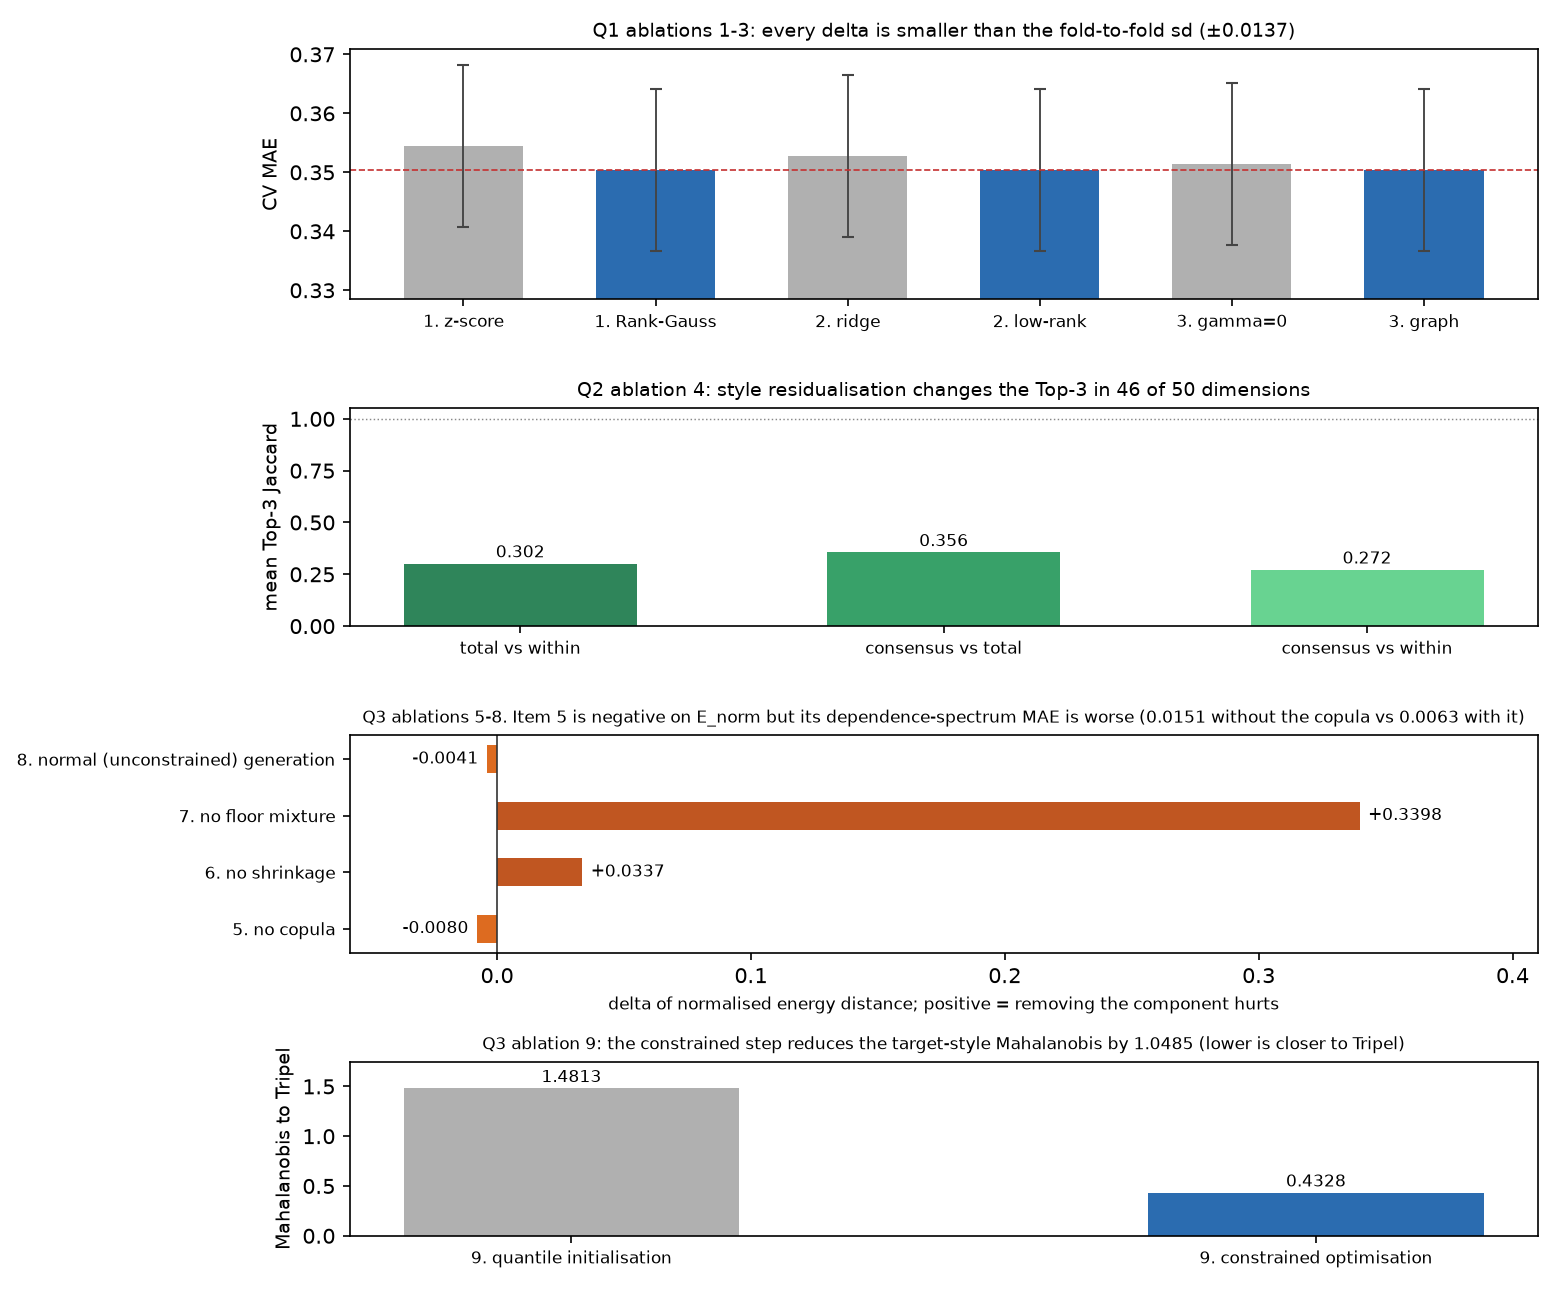
\includegraphics[keepaspectratio,alt={九项必做消融汇总（EXP-0035 从三个实验的产物重新汇总，本图即该审计实验的产物）。上：Q1 第 1--3 项消融两侧的训练内 CV MAE 与折间标准差，三个差值都小于折间波动；中：Q2 第 4 项消融的总关联/风格内关联/综合分的 Top-3 Jaccard；下左：Q3 第 5--8 项的能量距离差（第 5 项``无 Copula''能量距离反而低 0.0080，但依赖结构谱 MAE 0.0151 明显差于 0.0063）；下右：Q3 第 9 项分位数初始化与约束优化的目标马氏距离（1.481 → 0.433）。}]{../experiments/EXP-0035/figures/ablation-summary.png}}
\caption{九项必做消融汇总（EXP-0035
从三个实验的产物重新汇总，本图即该审计实验的产物）。上：Q1 第 1--3
项消融两侧的训练内 CV MAE 与折间标准差，三个差值都小于折间波动；中：Q2
第 4 项消融的总关联/风格内关联/综合分的 Top-3 Jaccard；下左：Q3 第 5--8
项的能量距离差（第 5 项``无 Copula''能量距离反而低 0.0080，但依赖结构谱
MAE 0.0151 明显差于 0.0063）；下右：Q3 第 9
项分位数初始化与约束优化的目标马氏距离（1.481 → 0.433）。}
\end{figure}

\subsection{9
结论、建议与局限}\label{ux7ed3ux8bbaux5efaux8baeux4e0eux5c40ux9650}

\textbf{结论}。(1) 在 50 维标准化感官标签上，训练内 OOF
融合相对逐目标中位数基线把留出 MAE 从 0.4005615400064 降到
0.3465674099243312（Skill
0.13479609170966855），而图正则与低秩约束本身只有弱增益；分级以训练折中点经验
CDF 定义并交付全部 250 行。(2) 每个感官维度的 Top-3 在风格分层 bootstrap
下并不唯一（\(\pi\) 均值 0.46468，无化合物
\(\pi=1\)），总体关联与风格内关联给出的答案显著不同（Jaccard
0.302），把风格混杂显式建模是必要的。(3) 风格条件 Copula
生成器在几乎不损失分布合理性的前提下把缺陷超阈率从与真实数据相当的 0.852
降到
0；跨风格迁移的「策略相对不恶化率」在四种情景下都等于可行域投影保证的上界，在「绝对不增」策略下「严格逐缺陷不增率」同样由约束构造保证，而在「超阈不恶化（cap-at-max）」策略下输出对严格不增的达标率只有
0.18181818181818182；两种策略的可行率与代价几乎相同，所以差别是\textbf{保证强度}而不是可行性，不能把该策略相对率读成经验性的可行性结论，也不能把该达标率读成``只有少数源样本可行''。

\textbf{建议}。对酿造实践，我们只提供\textbf{关联与生成合理性}层面的证据：不能把
Top-3 读成因果靶点；不能把 0--6
相对等级读成人工评分；生成的谱需要真实酿造与品评复核。若用于工艺优化，应先在小规模实验中检验``超阈不恶化''与``绝对不增''两种策略的实际代价。

\textbf{局限}（如实披露）。(i) 标签是 4.csv 标准化连续值，0--6
分级只是训练折参考分布下的相对量，且训练行的分级是 in-sample；(ii)
留出只有 50 行，单维估计的抽样波动不可忽略；(iii) 2.csv 与 6/7/8.xlsx
之间不是独立数据源，不能当作外部验证；(iv) Q3 的 t2n/stale hops 依赖 Q1
线性代理，代理 CV \(R^2\) 仅约 0.0548889784422808；(v)
小风格（Kriek、Lambic、Faro）区间很宽，不声称精确刻画；(vi) 缺陷阈值来自
8.xlsx 的汇总值，原文献的检出限与基质效应未逐条核对；(vii) Q3
稳健性判定阈值（25\%）较宽，已预注册并如实报告实际极差；(viii) 合并画像
Spearman 掩盖逐风格异质。

\subsection{附录 A
复现说明}\label{ux9644ux5f55-a-ux590dux73b0ux8bf4ux660e}

\begin{itemize}
\tightlist
\item
  环境：Python 3.12.14（numpy 2.3.5、pandas 2.2.3、scipy
  1.18.1、scikit-learn 1.9.1、matplotlib 3.11.2、openpyxl
  3.1.5）；所有实验由插件 runner 在 macOS Seatbelt 沙箱中执行，脚本只读
  \texttt{MODELING\_*} 指向的注册数据／划分与已登记依赖。
\item
  数据：\texttt{modeling\_data\ import} 导入 9 个附件并核对
  SHA256；\texttt{src/prepare\_base.py} 生成审计、尺度字典与
  \texttt{src/target\_columns.py}；\texttt{src/prepare\_q1mapped.py} 用
  SPLIT-0001 训练行生成 0--6 参考分级；\texttt{src/prepare\_q3.py} 生成
  Q3 视图与风格折协议。
\item
  顺序：init → probe → plan → 数据 → 契约 → 三问基线 → 逐问验证计划 →
  候选 → 验证（含独立复跑）→ 选定 → 稳健性（先登记后执行）→ 结论／覆盖 →
  审计（九项消融与 headline）→ 质量检查 → freeze → render → tex/pdf →
  artifact → check → package。
\item
  复现命令、种子与三处工程说明见 \texttt{REPRODUCE.md}；台账
  \texttt{state/ledger.json}
  记录每个实验的代码／数据／划分哈希与全部验证证据。
\end{itemize}

\subsection{附录 B
台账与证据索引}\label{ux9644ux5f55-b-ux53f0ux8d26ux4e0eux8bc1ux636eux7d22ux5f15}

\begin{itemize}
\tightlist
\item
  数据：DATA-0001（基准表）、DATA-0002（Q1 评估视图）、DATA-0003（Q3
  视图）、DATA-0004（Q3 leakage
  审计视图）；SPLIT-0001（训练行／映射／Q2）、SPLIT-0002（唯一 Q1
  评估划分）。
\item
  契约：TGT-0001（v2，labelSource 明确主分级规则）、TGT-0002（v2，50
  个目标列 + 219 单体分析宇宙 + 2.csv
  输入）、TGT-0003；MCON-0001（v3，主分级分段 AST + 7
  个边界样例）、MCON-0002、MCON-0003（v4，5 条数值约束 + 8
  个边界样例）。
\item
  关键实验：EXP-0001（Q1 基线）、EXP-0003/0004（Q1
  候选）、EXP-0002/0029（Q2）、EXP-0008/0033（Q3）、EXP-0016--0024（稳健性）、EXP-0026（250×50
  分级）、EXP-0035（九项消融审计）、EXP-0036（headline 审计）。
\item
  结论（每条一行，原文来自台账）：

  \begin{itemize}
  \tightlist
  \item
    在 SPLIT-0002 的 50 行留出上，训练内 OOF 融合（median 权重 0、graph
    0.649、HGB 0.351）把 50 维等权平均 MAE 从逐目标训练中位数基线的
    0.40056 降到 0.34657，R²=0.2317、相对基线的 Skill=0.1348，50 维中 38
    维改善、12 维恶化；同 seed 独立复跑（EXP-0010）在 1e-9
    容差内逐项复现全部 18 个指标键（VAL-0036）。该结论只适用于这 50
    行留出，是同期估计，不外推为未来预测。
  \item
    Q1 的三项训练内消融都只有很小的增益：Rank-Gauss
    相对原尺度标准化的训练内 CV MAE 低 0.00399，普通 Ridge
    相对低秩约束差 0.00232，γ=0 相对最优 γ=1 差
    0.00098，三者都小于折间标准差
    0.0137，因此不能声称图正则或低秩约束带来稳定增益。稳定的增益来自
    graph+HGB 的 OOF 融合（OOF MAE 0.3448，graph 单模型 0.3504，差
    0.0056）。这是负结果，按原样披露。
  \item
    在 200 行训练集上，以附件 2.csv 的 231×231 Spearman 矩阵（PSD
    投影：原始最小特征值 −0.0424，τ=0.5 时 644 条边、52
    个连通块）为附件描述网络、以训练集重算的 Spearman 图为正则化网络，50
    维 × 4 方法 Top-3 的平均两两 Jaccard 为 0.219（可由 sets.json
    原样复算），维度无关的全局 Top-3 基线为 0.20。500 次风格分层
    bootstrap 下交付 Top-3 的入选频率均值 0.465、没有任何化合物达到
    π=1。最终 Top-3 按蓝图 §4.4「π 优先、平均综合分 S
    裁决并列」给出（sets\_pi\_first.json）；把四个方法的 Top-3 全部换成
    π 优先重选结果后，同一 Jaccard 为 0.24，而点估计综合集口径仍为
    0.219，两者同时报告、不互相替换；π 优先集与点估计综合集的 Jaccard 为
    0.736。与 6.csv 独立 \textbar r\textbar{} 的秩相关均值 0.445（44/44
    化合物对齐）只支持方向一致性，不等同独立验证。只声明同期关联，不宣称因果或未来预测。
  \item
    风格条件 copula 生成器（κ=5、κ\_R=20，训练内跨折选择）在 310
    个输出（250 个 3 折 out-of-fold 生成 + 49 个 Tripel/Kriek/Lambic
    未见风格 + 11 个迁移）上按 MCON-0003 的五条声明式约束原生复算
    constraint-satisfaction=1.0（310/310）；未约束条件生成只有
    0.136，无条件全局高斯基线为 0.12。归一化能量距离由未约束的 0.2311
    升到 0.2352（同量真实---真实参照 0.1842，无条件基线
    0.7514）；缺陷超阈率由 0.852（真实数据 0.844）降到 0。50
    维合并感官画像 Spearman 为 0.796，但逐风格异质（Amber n=12
    为负、Kriek n=10 与 Strong ale n=18
    较高），合并分数不能读成逐风格可靠；t2n 与 stale\_hops 是 Q1
    线性代理（CV R² 0.055/0.050），只作弱证据。
  \item
    Pils/Lager→Tripel 迁移中，两种策略的\textbf{策略相对}非恶化率都是
    1.0，两种策略在「绝对不增」与 cap-at-max
    下的严格性差异如下：绝对不增策略（c\_new≤c\_source）的严格逐缺陷不增率为
    1.000，cap-at-max
    策略（c\_new≤max(c\_source,T)）的\textbf{严格达标率}为
    0.1818（逐缺陷：DMS 0.2727、2,3-butanedione 0.5455（mean
    阈值）/0.7273（median 阈值）、4VG 0.4545；t2n 与 stale\_hops 为 1.0
    但两者是 Q1 线性代理，CV R² 0.055/0.050）。四种情景的可行率都是
    1.000，平均 L1
    改动与目标马氏距离几乎相同，因此两种策略的差别是\textbf{约束保证的强度}（严格不增
    vs 不超过 max(source,T)），而不是可行性或代价上的张力；0.1818
    描述的是 cap-at-max 输出的严格达标比例，不能读成「只有 18.18\%
    的源样本存在严格不增可行解」。对 t2n/stale 两个代理约束做 100
    次标签代理重抽样，其联合非恶化率的 2.5\% 分位为
    0.2727（代理口径，不是五类缺陷严格率的下界）。约束优化把到 Tripel
    的马氏距离由分位数初始化的 1.481 降到 0.433，平均 L1 改动 7.19；mean
    与 median 两套阈值情景的目标距离几乎相同。
  \item
    三项预注册稳健性判定全部通过：Q1 训练内 CV MAE 在 seed 与 λ
    扰动下的相对极差 0.00447（≤0.03，ROB-0001 重算记录）；Q2
    topk-jaccard 在 seed 与 τ 扰动下相对极差 0（≤0.05，ROB-0002）；Q3
    归一化能量距离在 seed 与 κ 扰动下相对极差
    0.0827（≤0.25，ROB-0003），且 constraint-satisfaction 恒为 1.0。
  \end{itemize}
\item
  图：论文实际引用的 14 张为
  FIG-0016--FIG-0024、FIG-0026、FIG-0028、FIG-0029、FIG-0030、FIG-0031（Q1
  五张、Q2 三张、Q3 五张、九项消融汇总一张；FIG-0030/0031
  是图面修订后重新登记的缺陷超阈率图与 Pareto 图）。逐图 sha256
  入台账；被取代的 FIG-0025/0027 已用 figure-retire 标记为
  superseded（分别指向 FIG-0030/FIG-0031），旧字节归档到
  \texttt{figures/archive/FIG-0025-q3\_defect\_exceedance.png} 与
  \texttt{figures/archive/FIG-0027-q3\_pareto.png}（归档字节与登记
  sha256 逐字节核验一致），旧记录、路径历史与旧→新关系保留在台账。
\end{itemize}

\end{document}
